\documentclass[11pt,twoside,openright]{moddalthesis}

\usepackage{hyperref}

\usepackage[spanish,english]{babel}
%\usepackage[spanish]{babel}
%\usepackage[latin1]{inputenc}
\usepackage[utf8]{inputenc}
\usepackage{CJKutf8}


%-------------------------------------
\usepackage{chronology}
\usepackage{epigraph}

\usepackage{graphicx}
\usepackage{color}

\usepackage[symbols,nogroupskip,nonumberlist,sort=use]{glossaries-extra}


%\usepackage[backend=biber,style=alphabetic,citestyle=authoryear]{biblatex}

%\usepackage{natbib}    % Change bibstyle.

\usepackage{amsmath}
\usepackage{amsfonts}
\usepackage{amssymb}
%\usepackage{subfig}
\usepackage{subfigure} 

\usepackage{amsthm}
\theoremstyle{definition}
\newtheorem{definition}{Definition}[section]


\usepackage{booktabs}
\usepackage{siunitx}
\sisetup{math-micro=\text{µ},text-micro=µ}

%--------
\usepackage[many]{tcolorbox}
\usepackage{marginnote}
\usepackage{kantlipsum}
\tcbuselibrary{skins,breakable}
\newtcolorbox{story}[1][]{
    width=\textwidth,
    colback=magenta!20,
    colframe=red!75!black,
    colbacktitle=blue!85!black,
    fonttitle=\bfseries,
    left=0ex,
    right=0ex,
    top=0pt,
    arc=0pt,
    outer arc=0pt,
    leftrule=0pt,
    rightrule=0pt,
    toprule=0pt,
    bottomrule=0pt,
    breakable,
    enhanced jigsaw,
    title= #1}
\hypersetup{hidelinks=true}    
\usepackage{eso-pic}
\newcommand\AlCentroPagina[1]{% 
\AddToShipoutPicture*{\AtPageCenter{% 
\makebox(0,0){\hspace*{3cm}\includegraphics% 
[width=0.9\paperwidth]{#1}}}}}    
%-------

\newcommand{\blankpage}{
\newpage
\thispagestyle{empty}
\mbox{}
\newpage
}

\makenoidxglossaries

\glsxtrnewsymbol[description={Signal Segment Size}]{w}{\ensuremath{w}}
\glsxtrnewsymbol[description={Sample points}]{N}{\ensuremath{N}}
\glsxtrnewsymbol[description={Signal Span}]{lambda}{\ensuremath{\lambda}}
\glsxtrnewsymbol[description={Sampling Frequency}]{Fs}{\ensuremath{F_s}}
\glsxtrnewsymbol[description={Pixels in unit scale}]{Deltas}{\ensuremath{\Delta_s}}
\glsxtrnewsymbol[description={Peak-to-peak Amplitude}]{DeltamuV}{\ensuremath{\Delta \mu V}}
\glsxtrnewsymbol[description={Signal Amplitude Scale Factor}]{gamma}{\ensuremath{\gamma}}
\glsxtrnewsymbol[description={Time Scale Factor}]{gammat}{\ensuremath{\gamma_t}}
\glsxtrnewsymbol[description={Image Height}]{Hy}{\ensuremath{H_y}}
\glsxtrnewsymbol[description={Image Width}]{Wx}{\ensuremath{W_x}}
\glsxtrnewsymbol[description={Patch Horizontal Scale}]{St}{\ensuremath{S_t}}
\glsxtrnewsymbol[description={Patch Vertical Scale}]{Sv}{\ensuremath{S_v}}
\glsxtrnewsymbol[description={Patch Height}]{Sy}{\ensuremath{\mathbf{S}_y}}
\glsxtrnewsymbol[description={Patch Width}]{Sx}{\ensuremath{\mathbf{S}_x}}
\glsxtrnewsymbol[description={Keypoint}]{kp}{\ensuremath{\mathbf{kp}}}
\glsxtrnewsymbol[description={Pixel}]{P}{\ensuremath{\mathbf{p}}}


%$\gls{N}$, $\gls{\lambda}$, $\gls{F_s}$, $\gls{\Delta_s}$, $\gls{\Delta \mu V}$.

%\includeonly{FrontBackmatter/Contents,Chapters/Chapter03,Chapters/Chapter04,Chapters/Chapter05,Chapters/Chapter06,Chapters/Chapter0A,FrontBackmatter/Bibliography}

%\includeonly{Chapters/Chapter01,Chapters/Chapter02}

%-------------------------------------

%\addbibresource{Bibliography.bib}    % Use with biblatex

\begin{document}

\AlCentroPagina{images/itbalogoshaded}

\title{\textbf{Histogram of Gradient Orientations of EEG Signal Plots for Brain Computer Interfaces}}
\author{Rodrigo Ramele}
\dept{Doctorado}
\faculty{Escuela de Ingeniería en Informática}
\university{Instituto Tecnológico de Buenos Aires}
\address{Buenos Aires, Argentina}

\submitdate{30 de Noviembre, 2018}
\defencedate{Mes Día, 2018}
\copyrightyear{2018}
\convocation{Mes}{Año}

%\phd
\degree{Doctor en Ingeniería Informatica}
\degreeinitial{Doctor en Ingeniería Informatica}

\supervisor{Dr. Juan Miguel Santos}
\supervisor{Dra. Ana Julia Villar}

\firstreader{Dra. Jurado}
\secondreader{Dr. Jurado}
\thirdreader{Dr. Jurado}


%%% ZONA PARA LA PRIMERA PAGINA EN SP
%\title{\textbf{Titulo en Espanol}}
%\dept{Ingenier\'ia en Inform\'atica}
%\faculty{Ingenier\'ia}
%\university{Instituto Tecnol\'ogico de Buenos Aires}
%\address{Buenos Aires, Argentina}
%%
%\submitdate{Month Day, Year}
%\defencedate{Month Day, Year}
%\copyrightyear{Year}
%\convocation{Month}{Year}
% FINNNNN


\dedicate{\begin{CJK}{UTF8}{min}希望がある所に道もあります\end{CJK}}

%\nodedicationpage
%\notableofcontents
\nolistoftables
\nolistoffigures

%{
%\typeout{:?000000000} % Don't bother with over/under-full boxes
\beforepreface
%\typeout{:?111111111} % Process All Errors from Here on
%}

%\begin{abstract}
%Brain Computer Interface (BCI) or Brain Machine Interfaces (BMI), has proved the feasibility of a distinct non-biological communication channel to transmit information from the Central Nervous System (CNS) to a computer device.  Promising success has been achieved with invasive BCI, though biocompatibilities issues and the complexity and risks of surgical procedures are the main drive to enhance current non-invasive technologies.
%
%Electroencephalography (EEG) is the most widespread method to gather information from the CNS in a non-invasive way.  Clinical EEG has traditionally focused on temporal waveforms, but signal analysis methods which follow this path has been overshadow in BCI research. 
%
%This thesis propose a method and framework to analyze the waveform, the shape of the EEG signal, using the histogram of gradient orientations, a fruitful technique from Computer Vision which is used to depict image local characteristics. This method generates a feature, a 128-dimension descriptor, that  is used to to analyze the underlying cognitive phenomena. Inspiration comes from what traditionally electroencephalographers have been doing for almost a century: visually inspecting raw EEG signal plots. 
%
%The validity of the method is verified by identifying Visual Occipital Alpha Waves and Motor Imagery Rolandinc Mu rhythms. It is also applied on P300 ERP detection and used to implement a P300-Based Visual Speller application. Experimental protocols to produce these cognitive patterns were designed and own datasets produced and published using both commercial-grade and research-grade EEG devices.  Obtained results on public and own datasets are outlined, and comparisons performed against similar procedures.
%
%The benefits of the approach presented here are twofold, (1) it has a universal applicability because the same basic methodology can be applied to detect different patterns in EEG signals with applications to BCI and (2) it has the potential to foster close collaboration with physicians and electroencephalograph technicians because this direction of work follows the established procedure of the clinical EEG community of analyzing waveforms by their shapes.
%\end{abstract}


\begin{abstract}

Brain Computer Interface (BCI) or Brain Machine Interfaces (BMI), has proved the feasibility of a distinct non-biological communication channel to transmit information from the Central Nervous System (CNS) to a computer device.  Promising success has been achieved with invasive BCI, though biocompatibilities issues and the complexity and risks of surgical procedures are the main drive to enhance current non-invasive technologies.  

Electroencephalography (EEG) is the most widespread method to gather information from the CNS in a non-invasive way.  Clinical EEG has traditionally focused on temporal waveforms, but signal analysis methods which follow this path has been overshadow in BCI research. 

This thesis propose a method and framework to analyze the waveform, the shape of the EEG signal, using the histogram of gradient orientations, a fruitful technique from Computer Vision which is used to characterize image local features. Inspiration comes from what traditionally electroencephalographers have been doing for almost a century: visually inspecting raw EEG signal plots. 

This technique can be outlined in five steps, (1) signal preprocessing, (2) signal segmentation, (3) transformation on a channel by channel basis of each signal segment into a binary image of a signal plot, (4) assignment of keypoint location on a position over the newly created image depending on the physiological phenomena under study and finally (5) the calculation of the histogram of gradient orientations using finite differences from the image around this keypoint. This method generates a feature, a normalized 128-dimension descriptor. This feature is used to compare the signal segments that were used to generate them, hence to analyze the underlying cognitive phenomena. 

The validity of the method is verified by studying three cognitive patterns.  First, Visual Occipital Alpha Waves are analyzed.  An experimental protocol is designed and a dataset is produced using a commercial-grade EEG device.  Additionally, the ability of the method to capture oscillatory processes is verified by analyzing a public dataset. Moreover, this methodology is extended to study a related oscillatory process: Motor Imagery Rolandic Mu rhythms.  The performance of the method to discriminate right vs left motor imagery against a public dataset of healthy subjects, is verified.  Results are informed and reported. 

Finally, the method is modified to capture transient events, particularly the P300 Event Related Potential (ERP).  A description on how to extract the ERP from the EEG segment is offered, and a detailed depiction of how to implement a P300-Based BCI Speller application is outlined.  Its performance is verified by processing a public dataset of Amiotrophic Lateral Sclerosis (ALS) patients and contrasted against an own dataset produced in-house replicating the same experimental conditions.  Results are compared against other methods referenced in the bibliography

The benefits of the approach presented here are twofold, (1) it has a universal applicability because the same basic methodology can be applied to detect different patterns in EEG signals with applications to BCI and (2) it has the potential to foster close collaboration with physicians and electroencephalograph technicians because this direction of work follows the established procedure of the clinical EEG community of analyzing waveforms by their shapes.


%In recent years, the idea of a direct interface between the human brain and an artificial system, called Brain Computer Interface (BCI) or Brain Machine Interfaces (BMI), has proved the feasibility of a distinct non-biological communication channel to transmit information from the Central Nervous System (CNS) to a computer device. Its most important application is for people affected by neuro-degenerative diseases.
%
%Promising success has been achieved with invasive BCI, i.e. with surgically implanted electrodes, from the total reproduction of arm movement to the remote control of a manipulator by a macaque, using brainwave information. However, biocompatibilities issues and the complexity and risks of surgical procedures are the main drive to enhance current non-invasive technologies. 
%
%By estimates from the 2016 BCI Award, around 71.2$\%$ of noninvasive BCI research is based on non-invasive brain imaging modality, particularly Electroencephalography (EEG), which is the most widespread method to gather information from the CNS in a non-invasive way. EEG has been used in various working prototypes, as assisting devices, wheelchairs and speller applications. There have been many algorithms developed for processing EEG signals, based on time, frequency, spatial domains or combinations. However, the exploration of alternative procedures is ongoing, because non-invasive BCI still lacks the required performance to be used in real-time environments and to be ready for mainstream production.
%
%Although mature clinical EEG has traditionally focused on temporal waveforms, signal analysis methods which follow this path has been overshadow in BCI research. Hence, where are the waveforms ?
%
%%Few works have investigated the idea of exploiting signal waveforms to analyze the EEG signal on BCI applications. The seminal work of Bandt-Pompe Permutation Entropy [3] explores succinctly this concept and in [4] an approach based on Slope Horizontal Chain Code is presented. A similar methodology is implemented in [5] based on Mathematical Morphological Analysis. 
%
%This thesis propose a method and framework to analyze the waveform, the shape of the EEG signal, using the histogram of gradient orientations, a fruitful technique from Computer Vision which is used to characterize image local features. Inspiration comes from what traditionally electroencephalographers have been doing for almost a century: visually inspecting raw EEG signal plots. 
%
%%The validity of the method is verified by identifying and detecting Visual Occipital Alpha Waves and Motor Imagery Rolandinc Mu rhythms. It is also applied on P300 ERP detection and used to implement a P300-Based Visual Speller application.  Obtained results on public and own datasets are outlined and described. 
%
%This technique can be outlined in five steps, (1) signal preprocessing, (2) signal segmentation, (3) transformation on a channel by channel basis of each signal segment into a binary image of a signal plot, (4) assignment of keypoint location on a position over the newly created image depending on the physiological phenomena under study and finally (5) the calculation of the histogram of gradient orientations using finite differences from the image around this keypoint. This method generates a feature, a normalized 128-dimension descriptor. This feature is used to compare the signal segments that were used to generate them, hence to analyze the underlying cognitive phenomena. 
%
%The validity of the method was first verified studying three cognitive patterns.  First, Visual Occipital Alpha Waves are analyzed.  An experimental protocol is designed and a dataset is produced using a commercial-grade EEG device.  Additionally, the ability of the method to capture oscillatory processes is verified by analyzing a public dataset.
%
%Moreover, this methodology is extended to study a related oscillatory process: Motor Imagery Rolandic Mu rhythms.  The performance of the method to discriminate right vs left motor imagery against a public dataset of healthy subjects is verified.  Results are informed and reported.
%
%Finally, the method is modified to capture transient events, particularly the P300 Event Related Potential.  A detailed description on how to extract the ERP from the EEG segment is offered, and a detailed description of how to implement a P300-Based BCI Speller application is outlined.  It's performance is verified by processing a public dataset of ALS patients and contrasted against an own dataset produced in house replicating the same experimental conditions.
%
%%This novel procedure is biomimetically based on how the visual cortex works by detecting orientations, and ironically, is used here to detect information about how the brain works. 
%
%The benefits of the approach presented here are twofold, (1) it has a universal applicability because the same basic methodology can be applied to detect different patterns in EEG signals with applications to BCI and (2) it has the potential to foster close collaboration with physicians and electroencephalograph technicians because this direction of work follows the established procedure of the clinical EEG community of analyzing waveforms by their shapes.
%
%%Material, Methods and Results: The histogram of gradient orientations is a popular and powerful tool used in Computer Vision to characterize local features from images and is the basis of the feature generation algorithm in Lowe's SIFT Descriptor [7]. This technique can be applied to identify components in EEG signals in five steps, (1) signal preprocessing, (2) signal segmentation, (3) transformation on a channel by channel basis of each signal segment into a binary image of a signal plot, (4) assignment of keypoint location on the newly created image depending on the physiological phenomena under study and finally (5) calculation of the histogram of gradient orientations using finite differences from the image around the keypoint (Figure 1). This method generates a feature, a normalized 128-dimension SIFT descriptor, which can be used to compare the signal segments that were used to generate the plots, thus they can be used to analyze the underlying cognitive phenomena. 

%This method was used to identify and detect Visual Occipital Alpha Waves, Motor Imagery Rolandinc Mu rhythms [6] with results above chance level. It was also tested on P300 detection for Visual P300 Speller Matrix on ALS public dataset and for an own dataset of healthy subjects as well as identifying K-Complexes in sleep EEG (unpublished, under review). 
%
%Discussion: A procedure which is biomimetically based on how the visual cortex works by detecting orientations, ironically, is used precisely to detect information from the brain. Although we found that it is possible to decode with accuracy above chance level and to differentiate patterns with cognitive correlations, the stability of the signature of the component is a key and challenging aspect. The method was also applied to patterns which are more frequently studied by their spectral characteristics. 
%
%Significance: A method to analyze EEG signals which is based on the waveform characterization is presented. The benefits of the proposed approach are twofold, (1) it has a universal applicability because the same basic methodology can be applied to detect different patterns in EEG signals with applications to BCI and (2) it has the potential to foster close collaboration with physicians and electroencephalograph technicians because the approach follows the established procedure of the clinical EEG community of analyzing waveforms by their shapes.


%This thesis is a proposal of a new method to analyze and classify EEG (Electroencephalography) signals based on the extraction of characteristics based on the signal's waveform structure obtained from images of signal plots.  
%This procedure has the advantage that the features which are used to classify are visually relevant and meaningful to a human observer, particularly to a physician, improving close collaboration and clinical adoption.  
%Moreover, this may allow to tackle this demanding technology from a different perspective and improve the prospects of the BNCI, Brain Neural Computer Interaction field. 


%A very remarkable aspect of this communication channel is the ability to transmit some general cognitive state, like alertness, drowsiness, boredom, and so on, which can very helpful particularly in rehabilitation procedures.

%CNS's biosignals, like EEG, have a high variability between different subjects and even between different moments for the same subject. This inherent complexity is a real challenge when it is required to feasily extract information from raw EEG signals.
%
%Due to this inner complexity, it is often necessary to implement many distinct and specialized algorithmic methods, to filter the signal, classify it, and try to determine some meaning out of it.
%
%Outstanding success has been achieved with invasive BCI, i.e. with surgically implanted electrodes, from the total reproduction of arm movement to the remote control of a manipulator by a macaque using brainwave information. However, Biocompatibilities issues and the pervasive complexity and risks of surgical procedures are the main drive to enhance current non-invasive technologies. Above all, Electroencephalography (EEG), is the most widespread method to gather information from the CNS in a non-invasive way. It measures the summed activity of post-synaptic potentials from electrodes positioned over the scalp. EEG has been used in various working prototypes, as assisting devices, mainly wheelchairs. In order to derive information out of the subject's volition, different mental paradigms have been discovered and applied. There have been many algorithms developed so far for processing EEG signals, based on time, frequency, spatial domains or combinations. However, the exploration of alternative paths is ongoing, because non-invasive BCI still lacks the required performance to be used in real-time environments and to be ready for mainstream production.
%
%Those devices that not only restrict themselves to use CNSs signals, but they also include any kind of biological signal (EMG, EKG, EOG, GSR, etc) combined with sensor fussion algorithms are often called Hybrid BCIs or the BCI term is generalized to BNCI: Brain Neuronal Computer Interaction. Additionally, when the controlling device is not restricted to a computer, the term BMI, Brain Machine Interface, could be also used.

\end{abstract}

\newpage
\mbox{}
\newpage


\selectlanguage{spanish}%

\begin{abstract}

Las interfaces BCI (Brain Computer Interfaces, interfaces cerebro computadora) o BMI (Brain Machine Interfaces, interfaces cerebro máquina) han surgido como un nuevo canal de comunicación entre el cerebro y las computadoras, máquinas o robots, distinto de los canales biológicos estándar. Se han obtenido resultados prometedores en el empleo de la variante invasiva de BCI pero, además de los problemas de biocompatibilidad, los procedimientos quirúrgicos requeridos son complejos y riesgosos. Estas razones, han impulsado las mejoras de las tecnologías no invasivas.

La electroencefalografía (EEG) es el método más difundido para obtener información del sistema nervioso central de manera no invasiva.  La electroencefalografía clínica se ha enfocado tradicionalmente en el estudio de las formas de ondas temporales, pero los métodos de procesamiento de señales que exploren esta metodología han sido ignorados en las investigaciones sobre BCI.

Esta tesis propone un método y un marco para analizar las formas de las señales de EEG utilizando los histogramas de gradientes orientados, una técnica de visión por computadora que es utilizada para identificar y clasificar características locales en regiones de una imagen.  Este procedimiento está inspirado en lo que tradicionalmente los técnicos electroencefalógrafos han realizado por casi un siglo: inspeccionar visualmente los registros electroencefalográficos.

El método propuesto puede resumirse en 5 pasos, (1) preprocesamiento de la señal cruda, (2) segmentación de la señal, (3) obtención de una gráfica blanco y negro de la señal canal por canal, (4) asignación de una localización dentro de la imagen para posicionar un parche de un determinado tamaño y escala dependiendo del fenómeno cognitivo en estudio, y (5) cálculo del histograma de los gradientes orientados de la intensidades de los pixeles usando diferencias finitas.  Este mecanismo genera un vector de 128 dimensiones, que se utiliza para comparar los segmentos de señales entre sí, y que permite entonces analizar el fenómeno cognitivo subyacente.

La validez del método se verifica estudiando tres patrones cognitivos.  Primero se analizan las ondas alfa de la corteza visual occipital sobre dos conjuntos de registros: uno obtenido a partir de la aplicación de un protocolo experimental y mediante la utilización de un dispositivo electroencefalográfico digital de uso comercial, y otro obtenido de una base de datos pública de registros electroencefalográficos. Segundo, se analiza otro tipo de onda oscilatoria conocida como ritmo mu correspondiente a la corteza motora que puede ser también activada si el sujeto imagina una actividad motora.  Se reporta la efectividad del método para discriminar entre la actividad de la corteza motora derecha e izquierda en base al estudio de otro conjunto de registros público de pacientes sanos.  Los resultados son reportados y publicados.

Finalmente, el método propuesto se utiliza para estudiar eventos transitorios, particularmente, el potencial evocado P300.  La eficiencia del sistema es verificada mediante el procesamiento de un conjunto de registros público de pacientes con esclerosis lateral amiotrófica, y corroborada contra un conjunto de registros de sujetos sanos obtenidos de manera experimental, replicando el mismo protocolo. Para ambos conjuntos de registros, se realiza una descripción detallada de cómo extraer este potencial de la señal de EEG, y se implementa un procesador de texto basado en P300 para comparar el desempeño del método propuesto respecto de otros citados en la bibliografía.

Los beneficios de esta propuesta se resumen en, (1) tiene una aplicación potencialmente universal, debido  que el mismo tipo de metodología puede ser aplicada para detectar cualquier tipo de patrón obtenido en la señal de EEG con potenciales aplicaciones a BCI, y (2) ofrece la posibilidad de incentivar la colaboración y utilización de estas técnicas en la clínica médica especializada en electroencefalografía ya que esta perspectiva basada en el estudio de las formas de onda de las señales, es un procedimiento conocido y ya establecido por esa comunidad.

\end{abstract}

\selectlanguage{english} %

\begin{listofpubs}
%Lo reportado en las siguientes publicaciones conforma la base de la presente tesis.
The following publications are the basis of this thesis

\begin{itemize}
\item Ramele, R., A.J.Villar, and J.M.Santos."A Brain Computer Interface Classification Method Based on SIFT Descriptors." VI Latin American Congress on Biomedical Engineering CLAIB 2014, Paraná, Argentina 29,30,31 October 2014. Springer International Publishing, 2015.
\item Ramele, R., A. J. Villar, and J. M. Santos. "A Brain Computer Interface Classification Method Based on Signal Plots." 4th Winter Conference on Brain Computer Interfaces, Yongpyong, Korea, February 2016. IEEE Signal and Processing, 2016. 
\end{itemize}
\end{listofpubs}


\begin{acknowledgements}
Es un falacia creer que existe alguna actividad en nuestra vida que la hacemos solos.  Todos nosotros tenemos una interminable lista de personas a quienes le debemos agradecimiento, desde el primer segundo respirado hasta el último, y especialmente por aquellos actos ciclópeos que nos demandan todo lo que tenemos.
\end{acknowledgements}



\include{Chapters/Chapter_acronyms}
\addcontentsline{toc}{chapter}{List of Acronyms}

\listoftables
\addcontentsline{toc}{chapter}{List of Tables}

\listoffigures
\addcontentsline{toc}{chapter}{List of Figures}

\printnoidxglossary[type=symbols,style=long,title={List of Symbols}]
%$\gls{F}$, $\gls{t}$, $\gls{x}$, $\gls{v}$, $\gls{a}$.

\afterpreface
\linespread{1.5}
% ------------------------------------------------------------------------

%AQUI CHAPTERS

% \chapter[Introduction]{Introduction}
% ...
% \chapter[Future Work]{Future Work}

%\chapter*{Guia para mi - BORRAR}
%\addcontentsline{toc}{chapter}{Guia para mi} 
%
%Las tesis se tienen que escribir para alguno de estos tres:
%
%\begin{itemize}
%\item Neofito de BCI:  tesis larga, bastante completa y extendida.
%\item Para Wolpaw: 30 páginas aproximadamente, sólo con la propuesta.
%\item Para el Jurado: Focalizada
%\end{itemize}
%
%Esta tesis está escrita para el jurado con lo cual esta focalizada en el tema.  Sin embargo, tiene apéndices donde está información para un neofito de BCI  de Argentina.
%
%Esta tesis está estructurada de la siguiente forma
%
%\begin{itemize}
%\item Titulo
%\item Abstract: Español e Ingles
%\item Introduccion al propio manuscrito de la tesis
%\item State of the ART for BCI
%\begin{itemize}
%\item BCI
%\item EEG
%\item Abordaje BCI / EEG Basado en las waveforms
%\end{itemize}
%\item Histogram of oriented gradients of signal plots applied to bci
%\item Alpha Waves
%\item Motor Imagery
%\item P300
%\item Conclussions
%\item References
%\item Appendices
%\begin{itemize}
%\item Historia de BCI en Argentina (en castellano)
%\item SIFT
%\item Walkthrough de BCI
%\end{itemize}
%\end{itemize}
%
%Juliana's Tips:
%
%\begin{itemize}
%\item Por que este parrafo esta aca
%\item Ordenada
%\item Oraciones cortas
%\item Tiempo presente
%\item Items y descripciones una a una.
%\end{itemize}



\chapter*{Introduction}

During the last years of the 20th century an emerging idea took form and shaped one of the oldest dreams of mankind.

In terms of Schwartz Laboratory, the bandwidth of communication based on HCI devices seems very low (cite)

As mentioned in the most cited paper of the discipline, there are three motives behind BCI: the first is the Aging Societies: estimated for 2025, 800 millions people will be over 65 years old, and $2/3$ of them on developing countries.  This may lead to an increased tendency to develop diseases that affect motor pathways, that will require some for of assistance from technology. At the same time, science has provided the understanding that an Active Lifestyle is necessary to maintain body and mind health.  It is known that the ability to walk independently is a key indicator of psychological and physical health.   Last, but not least, the digital world demands more methods of interactions.  Digital society demands more mechanisms to interpret our surrounding  world and to translate our intentions through digital gadgets.

Objectives of this work

This thesis tries to unravel the following question:  it is possible to analyze and discriminate brainwaves signals, particularly Electroencephalographic signals, out of the automatic processing of the shape of waveforms using the Histogram of oriented gradients ?

To do that, I ask the reader to join me following this path:  (1) we will give details of what is Brain Computer Interfaces and the particularities of the first window of electric mind: the EEG.  (2)  we will cover also the state of the art in the methods that explore the waveform automatically.  The following section will give an overview about how a digital plotting is actually performed. The following section is the core of this theses and we will describe the Histogram of Gradient Orientations and how it can be used to process one dimensional signals.
Next, results and experimental procedures will be described, particularly Alpha Waves (4.3), Motor Imagery (5.2), P300 (6) and SSVEP.  Future Work and Conclussions will be addressed in 66.5.  Additionally, appendixes provide extra more information which is not extrictly related to this thesis but which provides information regarding the state-of-the-art of this discipline in Argentina, and also provides more inforamtion about the SIFT method and the theory behind the Histogram of Gradient Orientations of Signal Plots.



\chapter{Visually Decoding Brain Signals}

Where are the waveforms ? By estimates from the 2016 BCI Award, around 71.2$\%$ of noninvasive BCI research is based on Electroencephalography (EEG) [1]. Although mature clinical EEG has traditionally focused on temporal waveforms, and a whole branch of electrophenomenology has arisen around EEG graphoelements [2], signal analysis methods which follow this path has been overshadow in BCI research. Few works have investigated the idea of exploiting signal waveforms to analyze the EEG signal on BCI applications. The seminal work of Bandt-Pompe Permutation Entropy [3] explores succinctly this concept and in [4] an approach based on Slope Horizontal Chain Code is presented. A similar methodology is implemented in [5] based on Mathematical Morphological Analysis. The work proposed here is based on waveform analysis of the shape of the EEG signal, but using the histogram of gradient orientations, mimicking what traditionally electroencephalographers have been doing for almost a century: visually inspecting raw EEG signal plots. Material, Methods and Results: The histogram of gradient orientations is a popular and powerful tool used in Computer Vision to characterize local features from images and is the basis of the feature generation algorithm in Lowe's SIFT Descriptor [7]. This technique can be applied to identify components in EEG signals in five steps, (1) signal preprocessing, (2) signal segmentation, (3) transformation on a channel by channel basis of each signal segment into a binary image of a signal plot, (4) assignment of keypoint location on the newly created image depending on the physiological phenomena under study and finally (5) calculation of the histogram of gradient orientations using finite differences from the image around the keypoint (Figure 1). This method generates a feature, a normalized 128-dimension SIFT descriptor, which can be used to compare the signal segments that were used to generate the plots, thus they can be used to analyze the underlying cognitive phenomena. This method was used to identify and detect Visual Occipital Alpha Waves, Motor Imagery Rolandinc Mu rhythms [6] with results above chance level. It was also tested on P300 detection for Visual P300 Speller Matrix on ALS public dataset and for an own dataset of healthy subjects as well as identifying K-Complexes in sleep EEG (unpublished, under review). Discussion: A procedure which is biomimetically based on how the visual cortex works by detecting orientations, ironically, is used precisely to detect information from the brain. Although we found that it is possible to decode with accuracy above chance level and to differentiate patterns with cognitive correlations, the stability of the signature of the component is a key and challenging aspect. The method was also applied to patterns which are more frequently studied by their spectral characteristics. Significance: A method to analyze EEG signals which is based on the waveform characterization is presented. The benefits of the proposed approach are twofold, (1) it has a universal applicability because the same basic methodology can be applied to detect different patterns in EEG signals with applications to BCI and (2) it has the potential to foster close collaboration with physicians and electroencephalograph technicians because the approach follows the established procedure of the clinical EEG community of analyzing waveforms by their shapes.

Esta sección contiene el estado del arte del método

BCI + EEG

Cómo es el abordaje basado en Waveforms

Machine Learning

Shearlets

Scalar Space Theory


Diffusion Tensor Imagin

La idea es estructurar el paso a paso de como se puede ir usando el descriptor de gradientes de sift para 
mapear informacion.  Primero con una señal cruda, luego agregarle informacion extra, luego agregar ruido al azar, y finalmente empezar con información real de señales.  El tema luego se focaliza en EEG especificamente para BCI.


Describir la importancia de la impedencia (basado en el libro de Signal processing for neuro) con el paper que habla sobre EEG mas la pagina 144 del libro 2 de lotte.

Aca tambien pueden ir las referencias a la tesis de spinelli

Pattern Matching


Esta es la razon porque el metodo funciona ya que lo que termina detectando es de manera masiva
esas formas especificas que son las que le dan a las ondas alfa y mu sus nombres.

In human electrophysiology, oscillations with stereotyped nonsinusoidal shapes include the
sensorimotor mu rhythm, motor cortical beta oscillation, and cortical slow oscillations. The mu
rhythm oscillates at an alpha frequency (around 10 Hz) and was named because its waveform
shape resembles the Greek character m (Figure 1A). It is characterized by the fact that one
extremum (e.g., its peak) is consistently sharper than the other (e.g., its trough); it is also
described as an arch, comb, or wicket shape [4–10].
In addition to the sensorimotor mu rhythm, we have recently highlighted that motor cortical beta
oscillations also have striking nonsinusoidal features [11]. These beta oscillations manifest a
sawtooth shape in that their voltage either rapidly rises before more slowly falling off, or vice
versa (Figure 1B).


\section{EEG}

The EEG signal goes from 10-100 microvolts

monopolar, reference, averaged, 
bipolar

segmentation is commong, which is generally called epoching
trials are general realizations of the experiment.
tampering window could be gaussian, hamming, blackman, hanning

Impedance

\section{BCI}

A key contribution to this expansion has been the field of Brain Computer Interfaces (BCI)~\cite{WolpawJonathanR2012} which is the pursuit of the development of a new channel of communication particularly aimed to persons affected by neurodegenerative diseases.

One noteworthy aspect of this novel communication channel is the ability to transmit information from the Central Nervous System (CNS) to a computer device and from there use that information to control a wheelchair~\cite{Carlson2013}, as input to a speller application~\cite{Guger2009a}, in a Virtual Reality environment~\cite{Lotte2013} or as aiding tool in a rehabilitation procedure~\cite{Jure2016}.  The holly grail of BCI is to implement a new complete and alternative pathway to restore lost locomotion~\cite{WolpawJonathanR2012}.

EEG signals are remarkably complex and have been characterized as a multichannel non-stationary stochastic process.  Additionally, they have high variability between different subjects and even between different moments for the same subject, requiring adaptive and co-adaptive calibration and learning procedures~\cite{Clerc}.  Hence, this imposes an outstanding challenge that is necessary to overcome in order to extract information from raw EEG signals.

Moreover, EEG markers~\cite{Clerc} that can be used to  transmit volitional information are limited, and each one of them has a particular combination of appropriate methods to decode them. Inevitably, it is necessary to implement  distinct and specialized algorithmic methods, to filter the signal, enhance its Signal to Noise Ratio (SNR), and try to determine some meaning out of it.  

BCI has gained mainstream public awareness with worldwide challenge competitions like Cybathlon~\cite{Riener2014} and even been broadcasted during the inauguration ceremony of the 2014 Soccer World Cup.  New developments have overcome the out-of-the-lab high-bar and they are starting to be used in real world environments~\cite{Guger2017,Huggins2016}.  However, they still lack the necessary robustness, and its performance is well behind any other method of human computer interaction, including any kind of detection of residual muscular movement~\cite{Clerc}.

\begin{chronology}[5]{1983}{2010}{3ex}[\textwidth]
\event{1984}{one}
\event[1985]{1986}{two}
\event{\decimaldate{25}{12}{2001}}{three}
\end{chronology}

Where are we.
BCI plateau

BCNI Horizon, what the people is saying

Status in Argentina

Reference to thesis

OpenBCI and the Wearables movement

Neuro....everythig

\chapter{Signal Plots}

Contiene el método y el enfoque.

Mental Chrometry and averaging 
%https://www.ncbi.nlm.nih.gov/pmc/articles/PMC548951/



Broadly speaking, I would say there are three categories of neuroimaging: structural, functional, and chemical. These can then be subdivided into non-invasive, semi-invasive, and invasive, which delineate the degree of physical invasiveness involved in the imaging method. That is, cutting open the skull and implanting electrodes would be considered invasive, whereas putting the electrodes on the head (such as in scalp EEG) is non-invasive. Because I'm not proficient in animal imaging methods I will focus on human studies, most of which are non- or semi-invasive, with a few exceptions.

Structural Neuroimaging
Any technique that images structures of the brain. This would include CT (Computed Tomography), MRI (Magnetic Resonance Imaging), and DTI (Diffusion Tensor Imaging).

CT scanning is non-invasive uses x-rays to image tissue density. It is very rapid and can detect cerebral hemorrhaging in the early (acute) stage. It is most often, therefore, used for medical purposes.

Structural MRI is non-invasive and often provides better contrast resolution than CT with similar (and again, often better) spatial resolution. Unlike CT, structural MRI provides excellent tissue delineation, allowing users to visualize boundaries between grey and white matter in the brain, for example. Structural MRI is often used in neuroimaging to calculate volume of different brain regions or to define regions of brain damage or tumor.

DTI is non-invasive and can be done on most research MRI scanners. It involves using a special scanning and reconstruction sequence to image the flow (or, more specifically, constraints in the flow) of water through the brain. Because water flow is constrained by the axons (white matter) in the brain, it can be used to image large axonal connections between brain regions.


Functional Neuroimaging
Any technique that quantifies some metric of brain activity. This would include EEG (ElectroEncephaloGraphy), MEG (MagnetoEncephaloGraphy), fMRI (functional MRI), PET/SPECT (Positron Emission Tomography/Single Positron Emission Computed Tomography), NIRS (Near-InfraRed Spectroscopy), and, to a certain extent, TMS (Transcranial Magnetic Stimulation) and TDCS (Transcranial Direct Current Stimulation), along with several others.
\chapter{The Histogram of Oriented Gradients of Signal Plots}

In this section the generalities of the method will be described.

Image transformation and variants to transform a signal into an image.

sinuplot, spectrogram, scalogram


The research that encompass how to extract information 

The work of Edelman, Intrator and Poggio 1997 how the visual cortex sees features was the inspiration to the use of the histogram of gradient orientations to 


\chapter{Alpha Wave and Motor Imaginary: the power of masses}

First describe what are alpha waves

Describe the dataset generated

Describe how it was also used to test a public dataset.


\chapter{Alpha Wave: spotting wiggles}
\label{chapter:four}
\epigraph{The electroencephalogram represents a continuous curve with continuous oscillations in which... one can distinguish larger first order waves with an average duration of 90 milliseconds...}{Berger}

This Chapter describes the experiments performed over a well-established but still mysterious EEG cognitive signal: The Berger Rhythm or Visual Occipital Alpha Waves.  An own dataset of resting subjects with and without alpha blocking is produced and the details of their generation are outlined.  Additionally, an experiment on a public dataset is also delineated.  Conclusions and discussion are described in the last section.

\section{Introduction}

%We gather the first dataset  using the EEG EPOC Emotiv Headset and we  access the raw signals using its C++ SDK provided by the manufacturer.  The device sends wirelessly  digitalized 128 Hz sampled EEG information as discrete packets.  Every packet is numbered and the electronic impedance is constantly measured, and delivered as part of the packet information. The wireless transmitter connects to a standard RF dongle which receives the information from  14 channels and forwards it into the PC, particularly to a custom C++ EEG Datalogger program that was developed in-house.  The program is waiting passively until a new packet is received from the dongle, verifying the packet numbering and controlling that the impedance is bellow a certain level, according to the device's documentation \cite{Stopczynski2014}. 

Alpha Waves were the first signals ever spotted from the Electroencephalography.  They are regularly characterized as $10\si{Hz}$, or more broadly between the frequency band of $8$-$12$ $\si{Hz}$. They are physiologically consistent across subjects, though it has been reported inter- and intra- variations with functional cognitive implications~\cite{Haegens2014}.   Moreover, they are associated with synchronous inhibitory processes and attention shifting~\cite{c3}. They tend to be more prominent while subject's eyes are closed and appear stronger in occipital regions, around $O_1$ and $O_2$~\cite{WolpawJonathanR2012,Stopczynski2014}. These waves are also called Prominent Posterior Alpha or Posterior Dominant Rhythm due to their pervasiveness in EEG~\cite{Schomer2010,Haegens2014}.

Figure~\ref{fig:alphawavessignals} shows two records of 8-channels signals.  Figure ~\ref{fig:alphawavessignals}(a) contains the registered alpha waves of a subject with their eyes open while the (b) contains the same information with their eyes closed.  The characteristic pattern of wiggles can be spotted in the latter, while their absence entails the blocking of alpha waves in the former~\cite{Basar2012}. 


\begin{figure}[h!]
\centering
\subfigure[EEG signals of a relaxed healthy subject with their eyes open.]
{\includegraphics[height=5cm,width=7.5cm]{images/eeglab1.jpg}}
\subfigure[EEG signals of the same relaxed subject with their eyes closed. Alpha Waves wiggles can be spotted since the first second.]
{\includegraphics[height=5cm,width=7.5cm]{images/eeglab2.jpg}}
\caption[Alpha Waves Wiggles]{Five seconds of EEG signals obtained from the Emotiv EPOC device.  Fourteen channels are shown on the vertical axis, while x-axis shows time in seconds.}
\label{fig:alphawavessignals}
\end{figure}

This important rhythm is an oscillatory process.  As such, it is understood and studied in the frequency-domain.   Figure~\ref{fig:alphaspectrum} shows the results of applying the Fast Fourier Transform to two different segments of $10\si{\second}$ length.  For each segment, the power spectral density is calculated and their values are shown on the vertical axis.  Frequency values are shown on the horizontal axis.   On Figure (a) no particular frequency component can be spotted.  However, on Figure (b) the prevalence of the 10-\si{\hertz} alpha wave component can be observed.   
 
%As can be seen in Fig. , if we process the Drowsiness dataset with a 8-12Hz band-pass filter and calculate the average power spectral density across subjects and for each channel, we can see how clearly the value corresponding to class 2 (eyes closed) is always higher than the value for class 1 (eyes open), confirming the expected result.  This also verifies how the differentiation information is contained mostly in the frequency-domain.


%(Kamiya 1968) Neurofeedback controlling voluntarily.

\begin{figure}[h!]
\centering
\subfigure[Subject was sit, relaxed in front of the Computer Monitor with his eyes open.]
{\includegraphics[height=5cm,width=7.5cm]{images/spectrumeyesopenO2.jpg}}
%{\includegraphics[height=5cm,width=7.5cm]{images/eyesopen.eps}}
\subfigure[Subject was sit, relaxed in front of the Computer Monitor with his eyes closed. A strong $10 \si{Hz}$ component can be observed.]
{\includegraphics[height=5cm,width=7.5cm]{images/spectrumeyesclosedO2.jpg}}
%{\includegraphics[height=5cm,width=7.5cm]{images/eyesclosed.eps}}
\caption[Alpha Waves Spectrum Components]{Spectrum components of a $10 \si{s}$ signal segment of a subject with their eyes open. Horizontal axis shows different frequencies while the vertical axis represents the power spectral density.  In both diagrams a $50 \si{Hz}$ line component can be visualized.} 
\label{fig:alphaspectrum}
\end{figure}


%   \begin{figure}[thpb]
%      \centering
%      \setlength\fboxsep{0pt}
%	  \setlength\fboxrule{0.5pt}
%      \fbox{\includegraphics[width=2.5cm, height=1.8cm]{images/PSDExperiment1VsExperiment5.png}}
%      \fbox{\includegraphics[width=2cm, height=1.8cm]{images/s_1_e_1_c_7_4.png}}
%      \caption[Power Spectral Density of Alpha Waves]{PSD values for every channel (x-axis) are being shown for class 1, dashed line, and class 2, solid line, for Dataset I (left). Sample EEG plot image corresponding to the subject 1 (center) for class 1 (eyes open), for the channel 7 ($ O_1 $) }
%      \label{figure1}
%   \end{figure}
   
\section{Materials and Methods}

These experiments consist in performing a binary classification of EEG signal segments between the two defined classes.  Class 2 is assigned to segments containing significant alpha waves (i.e. eyes closed), whereas class 1 identifies those where these signals are blocked (i.e. eyes open).


\subsection{Dataset I - Emotiv EPOC alpha waves own dataset}
\label{dataset1}
The first dataset is gathered using the EEG EPOC Emotiv Headset.  Although this is a commercial-grade device, it provides an acceptable price-performance ratio and it has been used to investigate basic EEG processes~\cite{Debener2012,DeVos2014}. In order to obtain the multichannel raw EEG signal, a C++ SDK library provided by the manufacturer is used and an in-house software program is developed. This device has 14 channels, and a sampling rate of 128 \si{Hz}\cite{Stopczynski2014}. Available channels are AF3, F7, F3, FC5, T7, P7, O1, O2, P8, T8,  FC6, F4, F8, AF4.  Ten healthy subjects between ages 20-50 are recruited and they accept to wear the device and to participate in the experiments.  

A 30 minutes procedure is required to adjust the headset to each user, in order to decrease the impedance on each electrode (bellow $5 \si{\kilo\ohm}$).  
This is achieved by physically adjusting the headset position over the scalp, and by embedding each electrode electrode pad in saline solution.
A software program developed by the manufacturer is used to obtain the measured impedance.  Once the set up is finished, each subject is instructed to sit in a relaxed position. Subsequently, she/he is commanded to watch the screen for 15 seconds, trying to avoid, as much as possible, to abruptly move its body or head.  During that time, a single-trial of 10 seconds-length window of EEG signals data is transferred to a PC and logged into standard binary files. After a 5 minutes pause, the subject is asked to close the eyes avoiding any movement while keeping the same pose for another batch of 15 seconds.  Again, 10 seconds of EEG information are transferred and logged into the PC. This finally produces a dataset of 10 subjects,  2 classes per subject, composed of 14 channels, 10-seconds length or 1280 samples per window.  These windows are further divided into 10 segments per class and per subject.

%\begin{figure}[thpb]
%\centering
%\setlength\fboxsep{0pt}
%\setlength\fboxrule{0.5pt}
%\fbox{\includegraphics[width=3.5cm, height=2.5cm]{images/emotivlarge.png}}
%\fbox{\includegraphics[width=3.5cm, height=2.5cm]{images/emotivpositions.png}}
%\fbox{\includegraphics[width=3.5cm, height=2.5cm]{images/emotivcalibration.png}}
%\fbox{\includegraphics[width=3.5cm, height=2.5cm]{images/emotivdatasetsubject.jpg}}
%\caption[Classification Accuracy of Alpha Waves]{}
%\label{figure1}
%\end{figure}   
   
\begin{figure}[h!]
\centering
\subfigure[]
{\includegraphics[width=3.5cm, height=3cm]{images/emotivlarge.png}}
\subfigure[]
{\includegraphics[width=3.5cm, height=3cm]{images/emotivpositions.png}}
\subfigure[]
{\includegraphics[width=3.5cm, height=3cm]{images/emotivcalibration.png}}
\subfigure[]
{\includegraphics[width=3.5cm, height=3cm]{images/emotivdatasetsubject.jpg}}
\caption[EPOC Emotiv Alpha Waves Dataset]{(a)EPOC Emotiv consumer-grade 14-channels wireless EEG.(b) This device has a fixed set of positions according to the 10-20 International System.(c) While resting and sitting confortable in a chair, subjects had to fixate their sight to the center of this image which was being displayed on a computer monitor, 1 \si{meter} away from the subject.(d) Subject performing the experiment to produce the dataset described in \ref{dataset1}}.
\label{fig:alpharesults}
\end{figure}

      
\subsection{Dataset II - AlphaNet Dataset}
Additionally, the performance of HIST was tested against the public dataset EEG Motor Movement/Imagery Dataset of the PhysioNet effort published and mantained by the U.S. National Health Service~\cite{Schalk2004,Goldberger2000}.  

Baseline records and motor/imagery tasks were performed by 109 healthy volunteers, using the BCI2000 system~\cite{Schalk2004} at a sampling frequency $\gls{Fs} = 160$.  At the same time 64-channel EEG records were registered where each subject completed 14 tasks, called Runs.  The first two are the baseline calibration tasks, of relevance for this Chapter.  These Runs 1 and 2 are each one-minute records of resting subjects with eyes open and eyes closed.  From these records, 60 segments of 1-second length are further extracted per subject. Class labeling is the same as Dataset I.  The experiment was performed on 25 of the 109 subjects.


%This dataset
%
%Subjects performed different motor/imagery tasks while 64-channel EEG were recorded using the BCI2000 system (http://www.bci2000.org). Each subject performed 14 experimental runs: two one-minute baseline runs (one with eyes open, one with eyes closed), and three two-minute runs of each of the four following tasks:
%
%A target appears on either the left or the right side of the screen. The subject opens and closes the corresponding fist until the target disappears. Then the subject relaxes.
%A target appears on either the left or the right side of the screen. The subject imagines opening and closing the corresponding fist until the target disappears. Then the subject relaxes.
%A target appears on either the top or the bottom of the screen. The subject opens and closes either both fists (if the target is on top) or both feet (if the target is on the bottom) until the target disappears. Then the subject relaxes.
%A target appears on either the top or the bottom of the screen. The subject imagines opening and closing either both fists (if the target is on top) or both feet (if the target is on the bottom) until the target disappears. Then the subject relaxes.


\subsection{Parameters}

Images and plots are generated according to Section~\ref{Plot}, with an autoscale plotting scheme.  Keypoint localization is determined according to Section~\ref{keypointlocation} by following the trace of the signal, with a $\gls{kpd} = 1$.   Descriptors are extracted from all the generated images, from both classes, and they are used to classify images in a 10-fold cross-validation procedure.  The classification method described in Section~\ref{nbnn} is used to perform a binary classification.  The parameter $\gls{gamma}$ is set to $2$, as well as $\gls{gammat}$.  

%For the first two datasets, as the sampling frequency of both datasets is similar, Image and SIFT Descriptor Scale were adjusted to delta and gamma to 1.

%\subsection{Dataset III - BCI Competition 2003 IV \textit{self-paced 1s}}
%We validated our method against the "BCI Competition 2003, dataset IV \textit{self-paced 1s}" \cite{c51}. This dataset is composed of 28 channels, in 416 epochs of 50 samples per epoch (500 ms length at 100 Hz) each one with the corresponding label, where subjects were asked to type at will a letter on a keyboard with the right or left index finger.  It is based on the Bereitschaftspotential \cite{c52}, which is a Slow Cortical Potential, particularly a slow change in voltages towards a negative potential drift, around 1000-500 ms before the onset of the self-initiated movement.  In this case, the information lies strongly on the time-domain.
%
%This dataset was recorded from a healthy subject during a no-feedback session. She/he sat in a normal chair with relaxed arms resting on the table and fingers in the standard typing position at the computer keyboard. The task was to press with the index and little fingers the corresponding keys in a self-chosen order and timing 'self-paced key typing'. The experiment consisted of 3 sessions of 6 minutes each. All sessions were conducted on the same day with some minutes break in-between. Typing was done at an average speed of 1 key per second.  

\section{Results}

Dataset I was controlled and verified by processing it with a 8-12Hz band-pass filter, and calculating the average power spectral density across subjects for all channels.  It can be observed on Figure \ref{fig:psd}(a)  that values corresponding to class 2 (eyes closed) are always higher than the values obtained for class 1 (eyes open). On the other hand, for the sake of illustration, a scatter plot of the obtained segment's power spectral density for O1 vs O2 for Subject 2 is shown, where a separation of classes can be devised.  This proves that there is discriminative information in the frequency-domain.



\begin{figure}[h!]
\centering
\subfigure[Power spectral density averaged across 10 subjects for each channel. Values for Class 2 (red) are always higher than values for Class 1 (blue).]
{\includegraphics[width=7.5cm, height=5cm]{images/PSDExperiment1VsExperiment5.png}}
\subfigure[Scatterplot of power spectral density for the channel O1 vs O2.  There is a separation of classes between the red (class 2) and blue(Class 1) dots.]
{\includegraphics[width=7.5cm, height=5cm]{images/alphawavesscatterpsd.png}}
\caption[Power Spectral Density of the Dataset I]{Frequency analysis of Dataset I}
\label{fig:psd}
\end{figure}
   
Results of applying the 10-fold cross validation procedure on the entire set of labeled descriptors is shown on Figure~\ref{fig:alpharesultsdataseti}. Template Dictionaries for Class 1 and Class 2 are formed using training descriptors for all the subjects at the same time.  Hence, the testing step of the cross-validation procedure is implemented subject by subject, but performing a transfer learning between them. The classification is subject-independent, and an average above $70\%$ is obtained in occipital channels.
   
\begin{figure}[h!]
\centering
\subfigure[Ten-fold cross-validated accuracy values for $10$ subjects.  Descriptors were intermixed for all the subjects.]
{\includegraphics[width=7.5cm, height=5cm]{images/Dataset1AccuracyPerChannel}}
\subfigure[Sample descriptor patch located on one of the images generated for one 1-second long segment of this dataset.]
{\includegraphics[width=7.5cm, height=5cm]{images/AlphaWaveSampleEEG.png}}
\caption[Dataset I Classification Rate]{The classification accuracy is maximum on occipital channels O1 and O2. The horizontal patch scale $\gls{St}$ and the vertical patch scale $\gls{Sv}$ are set to $1$, whereas $\gls{gamma}$ and $\gls{gammat}$ are set to $2$, which corresponds to a variation of $\gls{DeltamuV} = 12$ microvolts in the signal amplitude during $\gls{lambda}=0.09$ $\si{seconds}$.}
\label{fig:alpharesultsdataseti}
\end{figure}

% Hay que traducir todo eso a los nuevos simbolos.
   

%  \begin{figure}[thpb]
%      \centering
%      \setlength\fboxsep{0pt}
%	  \setlength\fboxrule{0.5pt}
%      \fbox{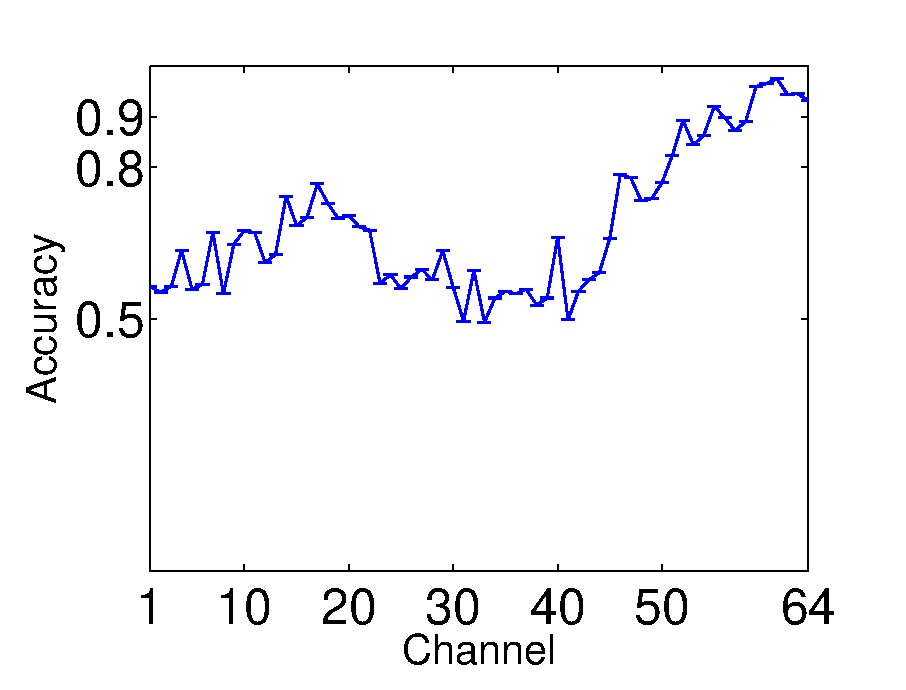
\includegraphics[width=7.5cm, height=5cm]{images/DatasetPhysionetAccuracyPerChannel}}
%      \fbox{\includegraphics[width=7.5cm, height=5cm]{images/DatasetPhysionetBoxPlots}}
%      \caption[Classification Accuracy of Alpha Waves]{}
%      \label{figure1}
%   \end{figure}   
   
\begin{figure}[h!]
\centering
\subfigure[Ten-fold cross-validated accuracies for O1, Oz, O2 and Iz channels for 25 subjects of the Alphanet Dataset. Medians are above $75\%$.]
{\includegraphics[width=7.5cm, height=5cm]{images/DatasetPhysionetBoxPlots}}
\subfigure[Ten-fold cross-validated accuracies values for subject number 12, using Runs 1 and 2 of the Alphanet Dataset.]
{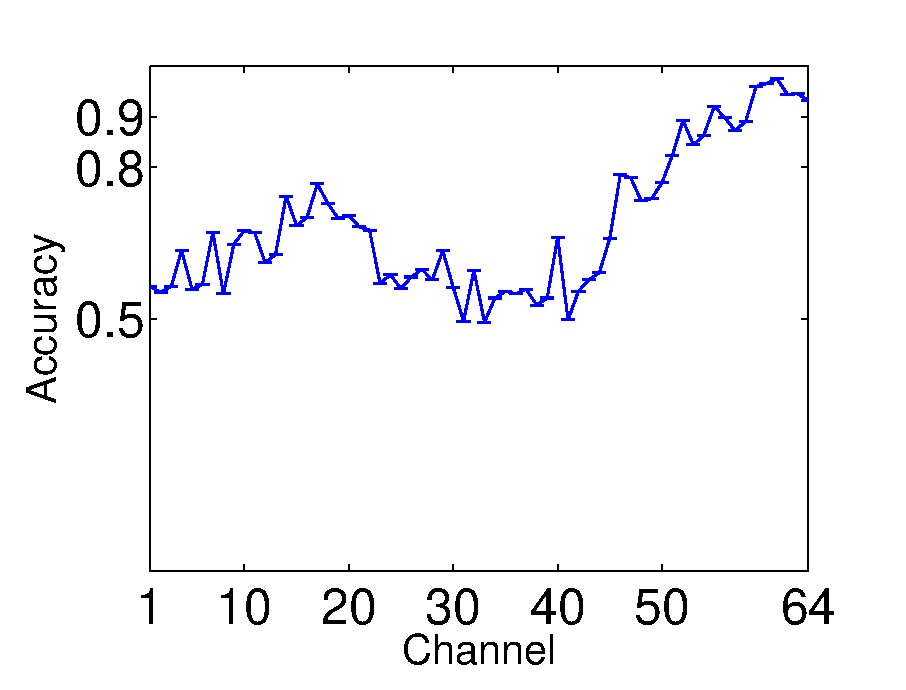
\includegraphics[width=7.5cm, height=5cm]{images/DatasetPhysionetAccuracyPerChannel}}
\caption[PhysioNet Dataset Classification Rate]{Classification Accuracy for segments of 1s ($\gls{N} = 160$) of EEG, between Class 1 and Class 2.}
\label{fig:alpharesultsdatasetii}
\end{figure}


For the Dataset II, training and testing steps of the cross-validation procedure are implemented subject by subject.  An accuracy median higher than $70\%$ for 25 subjects, also on occipital channels O1, Oz, O2 and Iz (numbered 61 to 64) is obtained while discriminating Runs 1 and 2 (Baseline eyes open vs Baseline eyes closed).  This information can be devised on Figure~\ref{fig:alpharesultsdatasetii}(a) where boxplots of the averaged classification accuracies for all the subjects are represented.  On the other hand, Figure~\ref{fig:alpharesultsdatasetii}(b) shows the 10-fold validated accuracy for one random subject. A higher accuracy in the classification of the signals can also be seen over occipital channels.

\section{Conclusion}

It is known and it was verified here that the discriminative information in EEG alpha waves is mostly contained in the frequency-domain.  In spite of this,  there is enough information encoded in the alpha waves wiggles to classify signal segments solely on the \textit{features} captured by the HIST method, proposed in this Thesis.  

It was also verified that the presence of oscillatory alpha waves is higher around occipital regions and that an automated procedure which analyze visually the image structure can detect them. This important oscillatory rhythm has many connections with shifting of attention and with volitional changes and is of quite relevance in BCI research.  Particularly, the BCI paradigm of Visual Spatial Covert Attention is a further area of research for this method due to the fact that it is entirely based on analyzing alpha waves. Moreover, the posterior rythm has many implications outside the field of BCI and is very important to assess healthy EEG patterns. The exact meaning of alpha waves is still debated\cite{Ahn2013} and this basic procedure can open the possibility to explore it under a different perspective and verify if they can be effectively tied to some unexpected form of volitional control which may be effective for BCI understanding and improvement.

%The key here is the classification algorithm that was used across this thesis.  This is because the local information obtained from each descriptor "help" to balance a tendency of how the synchronous waves all behave, and that information get loaded into the class structure that is later exploited by the classification method.
%
%This results was surprassing.  We are using a method which is based on the waveform do detect a process which happens to be more prominent in spectrum.  But this shows at the same time the complex relationshipt between time and frequency.  The shape in time of a an oscilatory process prominent in frequency is clearly evident.  This goes in line with the fact that alpha waves can be seen in the EEG, and are basic tools of clinical diagnosis.

%Although EPOC Emotiv is a commercial device, more apt as HCI tool, it is possible to detect fairly some BCI components.





\chapter{Event Related Potential: The P300 Wave}
\label{chapter:six}
\epigraph{This can be used to do this and that and that from Vidal paper!}{Vidal}

\section{Introduction}

The P300~\cite{Farwell1988,Knuth2006} is a positive deflection of the EEG signal which occurs around $300$ ms after the onset of a rare and deviant stimulus that the subject is expected to attend.  It is produced under the oddball paradigm~\cite{WolpawJonathanR2012} and it is consistent across different subjects. It has a lower amplitude  ($\pm 5 \mu V $) compared to basal EEG activity, reaching a Signal to Noise Ratio (SNR) of around $-15$ db estimated based on the amplitude of the P300 response signal divided by the standard deviation of the background EEG activity~\cite{Hu2010}.  This signal can be used to implement a speller application by means of a Speller Matrix~\cite{Farwell1988}. Fig.~\ref{fig:p300matrix} shows an example of the Speller Matrix used in the OpenVibe open source software~\cite{Renard2010}, where the flashes of rows and columns provide the deviant stimulus required to elicit this physiological response.   Each time a row or a column that contains the desired letter flashes, the corresponding synchronized EEG signal should also contain the P300 signature and by detecting it, the selected letter can be identified.


In response to this counting, a potential was elicited in the brain.  This response is kown as a P300 wave, as first reported by Sutton.  Detection of the responses an their timing in the measured signal made it possilbe to match rthe responses to one of the rows and one of the columns, and thus, the consen symbol cound be identified.

The flicker Effect (Neuro time series book) and their connection to SSVEP.  Verification of the dataset by means of SSVEP detection.

\section{Materias and Methods}

\subsection{Feature Extraction from Signal Plots} \label{Feature}

In this section, the signal preprocessing, the method for generating images from signal plots, the feature extraction procedure and the Speller Matrix identification are described.  Figure~\ref{fig:classification} shows a scheme of the entire process.

\subsubsection{Preprocessing Pipeline} \label{Pipeline}

The data obtained by the capturing device is digitalized and a multichannel EEG signal is constructed.

%A trial, as defined by the BCI2000 platform~\cite{Schalk2004}, is every attempt to select a letter from the speller. 

%It is composed of signal segments $S_{i}^l$ corresponding to $k_a$ repetitions of flashes of 6 rows and $k_a =10$ repetitions of flashes of 6 columns of the matrix, yielding 120 repetitions. 

The $6$ rows and $6$ columns of the Speller Matrix are intensified providing the visual stimulus.  The number of a row or column is a location. A sequence of twelve randomly permuted locations $l$ conform an intensification sequence. The whole set of twelve intensifications is repeated $k_a$ times.

%The multichannel EEG signal is processed on a channel by channel basis.   

\begin{itemize}
\item \textbf{Signal Enhancement}: This stage consists of the enhancement of the SNR of the P300 pattern above the level of basal EEG. The pipeline starts by applying a notch filter to the raw digital signal, a $4$th degree $10$ Hz lowpass Butterworth filter and finally a decimation with a Finite Impulse Response (FIR) filter of order $30$ from the original sampling frequency down to $16$ Hz \cite{Krusienski2006}.
\item \textbf{Artifact Removal}: For every complete sequence of $12$ intensifications of $6$ rows and $6$ columns, a basic artifact elimination procedure is implemented by removing the entire sequence when any signal deviates above/bellow $ \pm 70 \mu V $.
\item \textbf{Segmentation}: For each of the $12$ intensifications of one intensification sequence,  a segment $S_{i}^l$  of a window of $t_{max} $ seconds of the multichannel signal is extracted, starting from the stimulus onset, corresponding to each row/column intensification $l$ and to the intensification sequence $i$. As intensifications are permuted in a random order, the segments are rearranged corresponding to row flickering, labeled 1-6, whereas those corresponding to column flickering are labeled 7-12.  Two of these segments should contain the P300 ERP signature time-locked to the flashing stimulus, one for the row, and one for the column.
\item \textbf{Signal Averaging}: \label{Average}  The P300 ERP is deeply buried under basal EEG so the standard approach to identify it is by point-to-point averaging the time-locked stacked signal segments.  Hence the values which are not related to, and not time-locked to the onset of the stimulus are canceled out~\cite{Liang2008}.  

This last step determines the operation of any P300 Speller.  In order to obtain an improved signal in terms of its SNR,  repetitions of the sequence of row/column intensification are necessary.  And, at the same time, as long as more repetitions are needed, the ability to transfer information faster is diminished, so there is a trade-off that must be acutely determined.

The procedure to obtain the point-to-point averaged signal goes as follows:

\begin{enumerate}
\item \label{paso1}Highlight randomly the rows and columns from the matrix.  There is one row and one column that should match the letter selected by the subject.
\item  \label{paso2} Repeat step~\ref{paso1} $k_a$ times, obtaining the $1 \leq l \leq 12$ segments $S_1^l(n,c),\dots,S_{k_a}^l(n,c)$, of the EEG signal where the variables $1 \leq n \leq n_{max}$ and $1 \leq c \leq C$  correspond to sample points and channel, respectively. The parameter $C$ is the number of available EEG channels whereas $n_{max}=F_s \  t_{max}$ is the segment length and $F_s$ is the sampling frequency.  The parameter $k_a$ is the number of repetitions of intensifications and it is an input parameter of the algorithm.
\item \label{paso3} Compute the Ensemble Average by
\begin{equation}
x^l(n,c)= \frac{1}{k_a}\sum_{i=1}^{k_a}S_i^l(n,c) 
\label{averaging}
\end{equation}  
for $1 \leq n \leq n_{max}$ and for the channels $1 \leq c \leq C$.  This provide an averaged signal $x^l(n,c)$ for the twelve locations $ 1 \leq l \leq 12$.
\end{enumerate}
\end{itemize}


\subsubsection{Speller Matrix letter Identification}
\label{Classification}

\paragraph{P300 ERP Extraction}
Segments corresponding to row flickering are labeled 1-6, whereas those corresponding to column flickering are labeled 7-12.  The extraction process has the following steps:

\begin{itemize}
%\setcounter{enumi}{3}

\item \textbf{Step A:}\label{pasoa} First highlight rows and columns from the matrix in a random permutation order and obtain the Ensemble Average as detailed in steps~\ref{paso1}, \ref{paso2} and \ref{paso3} in Section \ref{Average}.
\item \textbf{Step B:}\label{paso4} Plot the signals $\tilde{x}^l(n,c)$,  $1 \leq n \leq n_{max}$, $1 \leq c \leq C $,  according Section~\ref{Plot} in order to generate the images $I^{(l,c)}$ for rows and columns $1 \leq l \leq 12$.

\item \textbf{Step C:} Obtain the descriptors $ \mathbf{d}^{(l,c)}$ for rows and columns from $I^{(l,c)}$  in accordance to the method described in Section~\ref{SIFT}. 

\end{itemize}

\paragraph{Calibration}

A trial, as defined by the BCI2000 platform~\cite{Schalk2004}, is every attempt to select just one letter from the speller.  A set of trials is used for calibration and once the calibration is complete it can be used to identify new letters from new trials.

During the calibration phase, two descriptors $ \mathbf{d}^{(l,c)}$ are extracted for each available channel, corresponding to the locations $l$ of a selection of one previously instructed letter from the set of calibration trials.  These descriptors are the P300 templates, grouped together in a template set called $ T^c $.   The set is constructed using the steps described in Section \ref{Average} and the steps A, B and C of the P300 ERP extraction process.

Additionally, the best performing channel, $bpc$ is identified based on the the channel where the best Character Recognition Rate is obtained.

\paragraph{Letter identification}

In order to identify the selected letter, the template set $T^{bpc}$ is used as a database.  Thus, new descriptors are computed and they are compared against the descriptors belonging to the calibration template set $T^{bpc}$.

\begin{itemize}

\item \textbf{Step D:} Match to the calibration template $T^{bpc}$ by computing  

\begin{equation}
\hat{row} = \arg \min_{l \in \{1,\dots,6\}} \sum_{q \in N_T(\mathbf{d}^{(l,bpc)})}^{} {\left\lVert q -  \mathbf{d}^{(l,bpc)} \right\rVert}  ^{2}
\label{eq:multiclassificationrow}
\end{equation}

\noindent and

\begin{equation}
\hat{col} = \arg \min_{l \in \{7,\dots,12\}} \sum_{q \in N_T(\mathbf{d}^{(l,bpc)})}^{} {\left\lVert q -  \mathbf{d}^{(l,bpc)} \right\rVert} ^{2}
\label{eq:multiclassificationcol}
\end{equation}

\noindent where $N_T(\mathbf{d}^{(l,bpc)})$  is defined as $N_T(\mathbf{d}^{(l,bpc)}) = \{\mathbf{d} \in T^{bpc} / $  is the k-nearest neighbor of $ \mathbf{d}^{(l,bpc)} \}$ for the best performing channel.  This set is obtained by sorting all the elements in $T^{bpc}$ based on distances between them and $\mathbf{d}^{(l,bpc)}$, choosing the $k$ with smaller values, with $k$ a parameter of the algorithm.  This procedure is based on the k-NBNN  algorithm~\cite{Boiman2008}.

\end{itemize}
By computing the aforementioned equations, the letter of the matrix can be determined from the intersection of the row $ \hat{row} $ and column $ \hat{col} $. 
Figure~\ref{fig:classification} shows a scheme of this process. 


\subsection{Experimental Protocol} \label{Protocol}

To verify the validity of the proposed framework and method, the public dataset 008-2014~\cite{Riccio2013} published on the BNCI-Horizon website~\cite{Brunner2014} by  IRCCS Fondazione Santa Lucia, is used. Additionally, an own dataset with the same experimental conditions is generated. Both of them are utilized to perform an offline BCI Simulation to decode the spelled words from the provided signals. 

The algorithm is implemented using  VLFeat~\cite{Vedaldi2010} Computer Vision libraries on MATLAB V2014a (Mathworks Inc., Natick, MA, USA). Furthermore, in order to enhance the impact of our paper and for a sake of reproducibility, the code of the algorithm has been made available at: https://bitbucket.org/itba/hist.

In the following sections the characteristics of the datasets and parameters of the identification algorithm are described. 


\subsubsection{P300 ALS Public Dataset} \label{ALSDataset}

The experimental protocol used to generate this dataset is explained in~\cite{Riccio2013} but can be summarized as follows:  8 subjects with confirmed diagnoses but on different stages of ALS disease, were recruited and accepted to perform the experiments. The Visual P300 detection task designed for this experiment consisted of spelling 7 words of 5 letters each, using the traditional P300 Speller Matrix~\cite{Farwell1988}. The flashing of rows and columns provide the deviant stimulus required to elicit this physiological response.  The first 3 words are used for calibration and the remaining 4 words, for testing with visual feedback.  A trial is every attempt to select a letter from the speller. It is composed of signal segments corresponding to $k_a =10$ repetitions of flashes of 6 rows and $k_a =10$ repetitions of flashes of 6 columns of the matrix, yielding 120 repetitions.  Flashing of a row or a column is performed for 0.125 s, following by a resting period (i.e. inter-stimulus interval) of the same length.  After 120 repetitions an inter-trial pause is included before resuming with the following letter.

The recorded dataset was sampled at 256 Hz and it consisted of a scalp multichannel EEG signal for electrode channels Fz, Cz, Pz, Oz, P3, P4, PO7 and PO8, identified according to the 10-20 International System,  for each one of the 8 subjects.   The recording device was a research-oriented digital EEG device (g.Mobilab, g.Tec, Austria) and the data acquisition and stimuli delivery were handled by the BCI2000 open source software~\cite{Schalk2004}.

In order to assess and verify the identification of the P300 response, subjects are instructed to perform a copy-spelling task. They have to fix their attention to successive letters for copying a previously determined set of words, in contrast to a free-running operation of the speller where each user decides on its own what letter to choose.

\subsubsection{P300 for healthy subjects}

We replicate the same experiment on healthy subjects using a wireless digital EEG device (g.Nautilus, g.Tec, Austria).  The experimental conditions are the same as those used for the previous dataset, as detailed in section~\ref{ALSDataset}.  The produced dataset is available in a public online repository~\cite{owndataset}.

Participants are recruited voluntarily and the experiment is conducted anonymously in accordance with the Declaration of Helsinki published by the World Health Organization.  No monetary compensation is handed out and all participants agree and sign a written informed consent.  This study is approved by the \textit{Departamento de Investigación y Doctorado, Instituto Tecnológico de Buenos Aires (ITBA)}.  All healthy subjects have normal or corrected-to-normal vision and no history of neurological disorders. The experiment is performed with 8 subjects, 6 males, 2 females, 6 right-handed, 2 left-handed, average age 29.00 years, standard deviation  11.56 years, range 20-56 years.

EEG data is collected in a single recording session. Participants are seated in a comfortable chair, with their vision aligned to a computer screen located one meter in front of them.  The handling and processing of the data and stimuli is conducted by the OpenVibe platform~\cite{Renard2010}. 

Gel-based active electrodes (g.LADYbird, g.Tec, Austria) are used on the same positions Fz, Cz, Pz, Oz, P3,P4, PO7 and PO8.  Reference is set to the right ear lobe and ground is preset as the AFz position.   Sampling frequency is slightly different, and is set to 250 Hz, which is the closest possible to the one used with the other dataset.

%Fz, Cz, P3, Pz, P4, PO7, PO8 and Oz. 

%8 gel-based active electrodes (g.LADYbird) + g.LADYbird (GND) + g.GAMMAearclip (REF) C3, Cz, C4, CPz, P3, Pz, P4, POz, GND: AFz, REF: right ear

\subsubsection{Parameters}

The patch size is $X_P = 12s \times 12s$ pixels, where $s$ is the scale of the local patch and it is an input parameter of the algorithm. The P300 event can have a span of $400$ ms and its amplitude can reach $ 10 \mu V $~\cite{Rao2013}.  Hence it is necessary to utilize a signal segment of size $t_{max} = 1$ second and a size patch $X_P$ that could capture an entire transient event. With this purpose in consideration, the $s$ value election is essential.

%necesitamos definir el valor de s en función de los parámetros de la señal, de modo tal que el parche cubra el evento completo.  
We propose the Equations~\ref{eq:mapping2} and~\ref{eq:mapping1} to compute the scale value in horizontal and vertical directions, respectively. 
\begin{equation}
s_x = \frac{ \gamma \;  \lambda \  F_s}{12}
\label{eq:mapping2}
\end{equation}

\begin{equation}
s_y= \frac{\gamma \; \Delta \mu V}{12} 
\label{eq:mapping1}
\end{equation}

\noindent where $ \lambda $ is the length in seconds covered by the patch, $ F_s $ is the sampling frequency of the EEG signal (downsampled to 16 Hz) and  $\Delta  \mu V $ corresponds to the amplitude in microvolts that can be covered by the height of the patch. The geometric structure of the patch forces a squared configuration, then we discerned that by using $ s =s_x =s_y = 3 $ and $ \gamma = 4 $,  the local patch and the descriptor can identify events of 9 $ \mu V $ of amplitude, with a span of $ \lambda = 0.56$ seconds.  This also determines that $ 1 $ pixel represents $ \frac{1}{\gamma}= \frac{1}{4} \mu V $ on the vertical direction and $\frac{1}{F_s \ \gamma}=\frac{1}{64}$ seconds on the horizontal direction. The keypoints  $\mathbf{p_k}$  are located at $ (x_{p_k}, y_{p_k} )= ( 0.55 F_s \ \gamma, z^l(c) )= (35,  z^l(c)) $ for the corresponding channel $c$ and location $l$ (see Equation~\ref{eq:zerolevel}).   In this way the whole transient event is captured. 
Figure~\ref{fig:patchgeometry} shows a patch of a signal plot covering the complete amplitude (vertical direction) and the complete span of the signal event (horizontal direction). 

Lastly, the number of channels $C$ is equal to $8$ for both datasets, and the number of intensification sequences $k_a$ is fixed to $10$.  The parameter $k$ used to construct the set $N_T(\mathbf{d}^{(l,c)})$ is assigned to $k=7$, which was found empirically to achieve better results.  In addition, the norm used on  Equations \ref{eq:multiclassificationrow} and \ref{eq:multiclassificationcol} is the cosine norm, and descriptors are normalized to $ \left[ -1, 1 \right] $.

\section{Results}

Table~\ref{tab:resultsals} shows the results of applying the Histogram of Gradient Orientations (HIST) algorithm to the subjects of the public dataset of ALS patients. The percentage of correctly spelled letters is calculated while performing an offline BCI Simulation.  From the seven words for each subject, the first three are used for calibration, and the remaining four are used for testing.  The best performing channel  $bpc$ is informed as well. The target ratio is $1:36$; hence theoretical chance level is $2.8\%$. It can be observed that the best performance of the letter identification method is reached in a dissimilar channel depending on the subject being studied.  Table~\ref{tab:resultsals} and~\ref{tab:resultsown} show for comparison the obtained performance rates using single-channel signals with the Support Vector Machine (SVM)~\cite{Scholkopf2001} classifier.  This method is configured to use a linear kernel.  The best performing channel, where the best letter identification rate was achieved, is also depicted.

%The spelled words are \textit{GATTO}, \textit{MENTE}, \textit{VIOLA} and \textit{REBUS}.

The Information Transfer Rate (ITR), or Bit Transfer Rate (BTR), in the case of reactive BCIs~\cite{WolpawJonathanR2012}  depends on the amount of signal averaging required to transmit a valid and robust selection.  Figure~\ref{fig:performance} shows the performance curves for varying intensification sequences for the subjects included in the dataset of ALS patients. It can be noticed that the percentage of correctly identified letters depends on the number of intensification sequences that are used to obtain the averaged signal.  Moreover, when the number of intensification sequences tend to 1, which corresponds to single-intensification character recognition, the performance is reduced. As mentioned before, the SNR of the P300 obtained from only one segment of the intensification sequence is very low and the shape of its P300 component is not very well defined.

In Table~\ref{tab:resultsown} the results obtained for 8 healthy subjects are shown.  It can be observed that the performance is above chance level. It was verified that HIST method has an improved performance at letter identification than SVM that process the signals on a channel by channel strategy (Wilcoxon signed-rank test, $p =  0.004$ for both datasets).

%In Tables~\ref{tab:resultsals} and~\ref{tab:resultsown} results for character recognition rates using single channel signals with the SVM~\cite{Scholkopf2001}  classification algorithm are also shown.    This algorithm was configured to use a linear kernel.  The best performing channel where the best letter identification rate was obtained is also depicted.

%The PE algorithm, which is also devised on a time-domain description of the waveform, was implemented according to \cite{Unakafova2013} and its parameters were adjusted as stated by \cite{Zanin2012}, with an \textit{order} of $2$ and a \textit{sliding window} of size $10$. 

Tables~\ref{tab:resultsalsswlda} and~\ref{tab:resultsownswlda} are presented in order to compare the performance of the HIST method versus a multichannel version of the Stepwise Linear Discriminant Analysis (SWLDA) and SVM classification algorithms for both datasets.  The feature was formed by concatenating all the channels~\cite{Krusienski2006}.  SWLDA is the methodology proposed by the ALS dataset's publisher. Since authors \cite{Riccio2013} did not report the Character Recognition Rate obtained for this dataset, we replicate their procedure and include the performance obtained with the SWLDA algorithm at letter identification.  It was verified for the dataset of ALS patients that it has similar performance  against other methods like SWLDA or SVM, which use a multichannel feature (Quade test with $p=0.55$) whereas for the dataset of healthy subjects significant differences were found (Quade test with $p=0.02$) where only the HIST method achieved a different performance than SVM (with multiple comparisons, significant difference of level $0.05$).

%It was verified for the dataset of ALS patients that it has similar performance  against other methods like SWLDA or SVM, which use a multichannel feature (Quade test with $p=0.55$) whereas for the dataset of healthy subjects significant differences where found (Quade test with $p=0.02$) where the HIST method achieved a better performance than SVM (with multiple comparisons, significant difference of level $0.05$).
 
%\subsection{Occipital Channels}

The P300 ERP  consists of two overlapping components: the P3a and P3b, the former with frontocentral distribution while the later stronger on centroparietal region~\cite{Polich2007}. Hence, the standard practice is to find the stronger response on the central channel Cz~\cite{Riccio2013}. However, \cite{Krusienski2006} show that the response may also arise in occipital regions.  We found that by analyzing only the waveforms, occipital channels PO8 and PO7 show higher performances for some subjects. 

%\subsection{Stability of the P300 shape}

As subjects have varying \textit{latencies} and \textit{amplitudes} of their P300 components, they also have a varying stability of the \textit{shape} of the generated ERP \cite{Nam2010}.  Figure~\ref{fig:p300templates} shows 10 sample P300 templates patches for patients 8 and 3 from the dataset of ALS patients. It can be discerned that in coincidence with the performance results, the P300 signature is more clear and consistent for subject 8 (A) while for subject 3 (B) the characteristic pattern is more difficult to perceive.

Additionally, the stability of the P300 component waveform has been extensively studied in patients with ALS \cite{SellersandEmanuelDonchin2006,TomohiroMadarame2008,Nijboer2009,Mak2012,McCane2015} where it was found that these patients have a stable P300 component, which were also sustained across different sessions.  In line with these results we do not find evidence of a difference in terms of the performance obtained by analyzing the waveforms (HIST) for the group of patients with ALS and the healthy group of volunteers (Mann-Whitney U Test, $p=0.46$). Particularly, the best performance is obtained for a subject from the ALS dataset for which, based on visual observation, the shape of they P300 component is consistently identified.

%\subsection{Descriptor Space and classification method}

It is important to remark that when applied to binary images obtained from signal plots, the feature extraction method described in Section \ref{SIFT} generates sparse descriptors.  Under this subspace we found that using the cosine metric yielded a significant performance improvement. On the other hand, the unary classification scheme based on the NBNN algorithm proved very beneficial for the P300 Speller Matrix.  This is due to the fact that this approach solves the unbalance dataset problem which is inherent to the oddball paradigm~\cite{Tibon2015}.  

%Using the same feature but with classification methods SVM, feed forward Neural Networks and SWLDA  common in BCI Research achieved a reduced performance.

\section{Conclusion}

%In this paper, a new unsupervised method to enhance evoked response by target stimuli in an oddball paradigm was presented. Only given the time indexes of rows/columns intensifications, the proposed algorithm estimates the main components of the P300 subspace by providing the best SNR. It was shown to efficiently improve the quality of the evoked responses by taking into account the signal and the noise, as opposed to principal component analysis, which only considers the signal. Using this method to enhance P300 subspace before the BCI classification task speeds up the BCI since less words are required to train the spatial filters and the linear classifier, given a certain percentage of good symbol prediction. Moreover, using this spatial enhancement significantly reduces the dimension of the feature vector used to predict words.


%For both datasets, the experimental protocol uses a very short inter-stimulus interval which has the potential to increase the ITR but at the same time it reduces the amplitude of the P300 response, hence it may be more difficult to detect it~\cite{Rao2013}.   It is known that ISI alters the P300 amplitude and may affect the chance to detect the ERP.

%In the case of the P300 response, the oddball paradigm requires that one of the stimuli be infrequent. Hence this forces the data to be unbalanced~\cite{Tibon2015}.  At the same time, the NBNN method suffers from biased classification on unbalanced classes~\cite{Fornoni2014}. %Para solucionar este problema, 

Among other applications of Brain Computer Interfaces, the goal of the discipline is to provide communication assistance to people affected by neuro-degenerative diseases, who are the most likely population to benefit from BCI systems and EEG processing and analysis.

In this work, a method to extract an objective metric from the waveform of the plots of EEG signals is presented.  Its usage to implement a valid P300-Based BCI Speller application is expounded.  Additionally, its validity is evaluated using a public dataset of ALS patients and an own dataset of healthy subjects. 

%The method works on a channel by channel basis; in this way the best performing channel can be identified and used it to reduce the number of required EEG electrodes, leading to the development of more ergonomic capturing device.

It was verified that this method has an improved performance at letter identification than other methods that process the signals on a channel by channel strategy, and it even has a comparable performance against other methods like SWLDA or SVM, which uses a multichannel feature.
Furthermore, this method has the advantage that shapes of waveforms can be analyzed in an objective way.  We observed that the shape of the P300 component is more stable in occipital channels, where the performance for identifying letters is higher.   We additionally verified that ALS P300 signatures are stable in comparison to those of healthy subjects.

%Further work should be conducted over larger samples to cross-check the validity of these results.

We believe that the use of descriptors based on histogram of gradient orientation, presented in this work, can also be utilized for deriving a shape metric in the space of the P300 signals which can complement other metrics based on time-domain as those defined by~\cite{Mak2012}. It is important to notice that the analysis of waveform shapes is usually performed in a qualitative approach based on visual inspection~\cite{SellersandEmanuelDonchin2006}, and a complementary methodology which offer a quantitative metric will be beneficial to these routinely analysis of the waveform of ERPs.

%and, based on this idea, we wanted to complement the methodology with a cuantitative and objective sight

The goal of this work is to answer the question if a P300 component could be solely determined by inspecting automatically their waveforms.  We conclude affirmatively, though two very important issues still remain:

First, the stability of the P300 in terms of its shape is crucial: the averaging procedure, montages, the signal to noise ratio and spatial filters all of them are non-physiological factors that affect the stability of the shape of the P300 ERP.  We tested a preliminary approach to assess if the morphological shape of the P300 of the averaged signal can be stabilized by applying different alignments of the stacked segments (see Figure~\ref{fig:classification}) and we verified that there is a better performance when a correct segment alignment is applied.  We applied Dynamic Time Warping (DTW)~\cite{Casarotto2005} to automate the alignment procedure but we were unable to find a substantial improvement.  Further work to study the stability of the shape of the P300 signature component needs to be addressed.

The second problem is the amplitude variation of the P300. We propose a solution by standardizing the signal, shown in Equation~\ref{eq:standarizedaverages}. It has the effect of normalizing the peak-to-peak amplitude, moderating its variation. It has also the advantage of reducing noise that was not reduced by the averaging procedure.   It is important to remark that the averaged signal variance depends on the number of segments used to compute it \cite{van2006signal}.  The standardizing process converts the signal to unit signal variance which makes it independent of the number $k_a$ of signals averaged.   Although this is initially an advantageous approach, the standardizing process reduces the amplitude of any significant P300 complex diminishing its automatic interpretation capability.

In our opinion, the best benefit of the presented method is that a closer collaboration of the field of BCI with physicians can be fostered \cite{Chavarriaga2017}, since this procedure intent to imitate human visual observation.  Automatic classification of patterns in EEG that are specifically identified by their shapes like K-Complex, Vertex Waves, Positive Occipital Sharp Transient~\cite{Hartman2005} are a prospect future work to be considered. We are currently working in unpublished material analyzing K-Complex components that could eventually provide  assistance to physicians to locate these EEG patterns, specially in long recording periods, frequent in sleep research~\cite{Michel2012}.  
Additionally, it can be used for artifact removal which is performed on many occasions by visually inspecting signals.  This is due to the fact that the descriptors are a direct representation of the shape of signal waveforms. In line with these applications,  it can be used to build a database~\cite{Chavarriaga2017} of quantitative representations of waveforms and improve atlases~\cite{Hartman2005}, which are currently based on qualitative descriptions of signal shapes.


%The spelled words are \textit{GATTO}, \textit{MENTE}, \textit{VIOLA} and \textit{REBUS}.

\begin{table}[htb]
\caption[Single Channel Character Recognition Rates for ALS patient's Dataset]{Character recognition rates for the public dataset of ALS patients using the Histogram of Gradient (HIST) calculated from  single-channel plots.  Performance rates using single-channel signals with the SVM classifier are shown for comparison.  The best performing channel $bpc$ for each method is visualized}
\centering
%% \tablesize{} %% You can specify the fontsize here, e.g.  \tablesize{\footnotesize}. If commented out \small will be used.
\begin{tabular}{c|cc|cc}
\toprule
\textbf{Participant}	&  $bpc$ 	&  HIST &  $bpc$	&  Single Channel SVM \\
\midrule
1     &     Cz   &   $35\%$    &  Cz   & $15\%$   \\
2     &     Fz   &   $85\%$      &  PO8   & $25\%$   \\
3     &     Cz   &   $25\%$    &  Fz   & $5\%$   \\
4     &     PO8 &   $55\%$   &  Oz   & $5\%$    \\
5     &     PO7 &   $40\%$    &  P3   & $25\%$   \\
6     &     PO7 &   $60\%$  &  PO8   & $20\%$    \\
7     &     PO8 &   $80\%$   &  Fz   & $30\%$     \\
8     &     PO7 &   $95\%$     &  PO7   & $85\%$ \\

%\bottomrule
\end{tabular}
\label{tab:resultsals}
\end{table}

%The spelled words are \textit{MANSO},\textit{CINCO},\textit{JUEGO} and \textit{QUESO}.

\begin{table}[htb]
\caption[Single Channel Character Recognition Rates for Healthy Subject's Dataset]{Character recognition rates for the own dataset of healthy subjects using the Histogram of Gradient (HIST) calculated from  single-channel plots.  Performance rates using single-channel signals with the SVM classifier are shown for comparison.  The best performing channel $bpc$ for each method is visualized.}
\centering
%% \tablesize{} %% You can specify the fontsize here, e.g.  \tablesize{\footnotesize}. If commented out \small will be used.
\begin{tabular}{c|cc|cc}
\toprule
\textbf{Participant}	&  $bpc$	&  HIST &  $bpc$	&  Single Channel SVM \\
\midrule
1     &     Oz   &   $40\%$  &  Cz   &  $10\%$    \\
2     &     PO7   &   $30\%$      &  Cz   & $5\%$   \\
3     &     P4   &   $40\%$    &  P3   & $10\%$    \\
4     &     P4 &   $45\%$    &  P4   & $35\%$     \\
5     &     P4 &   $60\%$  &  P3   & $10\%$     \\
6     &     Pz &   $50\%$ &  P4   & $25\%$     \\
7     &     PO7 &   $70\%$  &  P3   & $30\%$     \\
8     &     P4 &   $50\%$    &  PO7   & $10\%$    \\

%\bottomrule
\end{tabular}
\label{tab:resultsown}
\end{table}


\begin{table}[htb]
\caption[Character Recognition Rates for ALS patient's dataset]{Character recognition rates and the best performing channel $bpc$ for the public dataset of ALS patients using the Histogram of Gradient (HIST) (repeated here for comparison purposes). Performance rates obtained by SWLDA and SVM classification algorithms with a multichannel concatenated feature.}
\centering
%% \tablesize{} %% You can specify the fontsize here, e.g.  \tablesize{\footnotesize}. If commented out \small will be used.
\begin{tabular}{c|cc|c|c}
\toprule
%\textbf{Participant}	&  \textbf{BPC}	& \multicolumn{2}{c}{Character Recognition Rates}\\
%\cline{1-5} \\
\textbf{Participant}	&  $bpc$	&  HIST & Multichannel SWLDA & Multichannel SVM \\
                                    &  for HIST        &           &                                       &   \\
\midrule
1     &     Cz   &   $35\%$  & $45\%$  & $40\%$\\
2     &     Fz   &   $85\%$  & $30\%$   & $50\%$   \\
3     &     Cz   &   $25\%$  & $65\%$ & $55\%$   \\
4     &     PO8 &   $55\%$ & $40\%$  & $50\%$   \\
5     &     PO7 &   $40\%$ & $35\%$  & $45\%$   \\
6     &     PO7 &   $60\%$ &  $35\%$  & $70\%$   \\
7     &     PO8 &   $80\%$ & $60\%$   & $35\%$   \\
8     &     PO7 &   $95\%$  & $90\%$   & $95\%$  \\

%\bottomrule
\end{tabular}
\label{tab:resultsalsswlda}
\end{table}

\begin{table}[htb]
\caption[Character Recognition Rates for Healthy Subject's Dataset]{Character recognition rates and the best performing channel $bpc$ for the own dataset of healthy subjects using the Histogram of Gradient (HIST) (repeated here for comparison purposes).   Performance rates obtained by SWLDA and SVM classification algorithms with a multichannel concatenated feature.}
\centering
%% \tablesize{} %% You can specify the fontsize here, e.g.  \tablesize{\footnotesize}. If commented out \small will be used.
\begin{tabular}{c|cc|c|c}
\toprule
%\textbf{Participant}	&  \textbf{BPC}	& \multicolumn{2}{c}{Character Recognition Rates}\\
%\cline{1-5} \\
\textbf{Participant}	&  $bpc$ 	&  HIST & Multichannel SWLDA & Multichannel SVM  \\
                                    &  for HIST        &           &                                       &   \\
\midrule
1     &     Oz   &     $40\%$  &     $65\%$  &     $40\%$ \\
2     &     PO7   &     $30\%$ &   $15\%$  &     $10\%$ \\
3     &     P4   &     $40\%$ &     $50\%$  &     $25\%$ \\
4     &     P4   &     $45\%$ &     $40\%$  &     $20\%$ \\
5     &     P4   &      $60\%$ &    $30\%$  &     $20\%$ \\
6     &     Pz   &      $50\%$ &    $35\%$  &     $30\%$ \\
7     &     PO7   &      $70\%$ &  $25\%$  &     $30\%$ \\
8     &     P4   &      $50\%$ &    $35\%$  &     $20\%$ \\

%\bottomrule
\end{tabular}
\label{tab:resultsownswlda}
\end{table}


\begin{figure}[h!]
\centering
\includegraphics[width=15cm]{images/openvibep300matrix.png}
\caption[P300 Speller Matrix]{Example of the $6 \times 6$ Speller Matrix used in the study obtained from the OpenVibe software.  Rows and columns flash in random permutations.}
\label{fig:p300matrix}
\end{figure}

\begin{figure}[h!]
\centering
\includegraphics[width=15cm]{images/classificationgraph.pdf}
\caption[P300 Speller Matrix Letter Identification]{For each column and row, an averaged, standardized and scaled signal $\tilde{x}^l(n,c)$ is obtained from the segments $S_i^l$  corresponding to the $k_a$ intensification sequences with $ 1 \leq i \leq k_a $ and location $l$ varying between $1$ and $12$. From the averaged signal, the image $I^{(l,c)}$ of the signal plot is generated and each descriptor is computed.  By comparing each descriptor against the set of templates, the P300 ERP can be detected, and finally the desired letter from the matrix can be inferred.}
\label{fig:classification}
\end{figure}

\begin{figure}[h!]
\centering
\includegraphics[width=16cm]{images/gradients.png}\label{samplegradients}
\caption[Histogram of Gradient Orientations for ERP]{ (A) Example of a plot of the signal, a keypoint and the corresponding patch. (B) A scheme of the orientation's histogram computation.  Only the upper-left four blocks are visible.  The first eight orientations of the first block, are labeled from $1$ to $8$ clockwise. The orientation of the second block $ B_{1,2} $ is labeled from $9$ to $16$.  This labeling continues left-to-right, up-down until the eight orientations for all the sixteen blocks are assigned. They form the corresponding descriptor of $128$ coordinates.  The length of each arrow represent the value of the histogram on each direction for each block. (C) Vector field of oriented gradients.  Each pixel is assigned an orientation and magnitude calculated  using finite differences. }
\label{fig:sampledescriptor}
\end{figure}

\begin{figure}[h!]
\centering
\includegraphics[width=10cm]{images/patchgeometry.pdf}
\caption[Patch Geometry]{The scale of local patch is selected in order to capture the whole transient event.  The size of the patch is $X_p \times X_p$ pixels. The vertical size consists of $4$ blocks of size $3 s_y$ pixels which is high enough as to contain the signal $\Delta  \mu V $, the peak-to-peak amplitude of the transient event. The horizontal size includes $4$ blocks  of $3 s_x$ and covers the entire duration in seconds of the transient signal event, $ \lambda $.   }
\label{fig:patchgeometry}
\end{figure}

\begin{figure}[h!]
\centering
\includegraphics[width=10cm]{images/performance.eps}
\caption[P300 Performance Curves]{Performance curves for the eight subjects included in the dataset of ALS patients.  Three out of eight subjects achieved the necessary performance to implement a valid P300 speller.}
\label{fig:performance}
\end{figure}


\begin{figure}[h!]
\centering
\includegraphics[width=15cm]{images/subject.png}\label{subject8}
\caption[Sample P300 Patches]{Ten sample P300 template patches for subjects 8 (A) and 3 (B) of the ALS Dataset.  Downward deflection is positive polarity. }
\label{fig:p300templates}
\end{figure}

\begin{figure}[h!]
\centering
\includegraphics[width=15cm]{images/boxplots.png}
\caption[P300 Classification Boxplots]{Obtained boxplots for the given algorithms.}
\label{fig:boxplots}
\end{figure}

\chapter{Event Related Potential: The P300 Wave}
\label{chapter:six}
\epigraph{Talking off the top of your head....}{Farwell and Donchin}

\section{Introduction}

The P300~\cite{Bashore1991,Farwell1988,Knuth2006} is a positive deflection of the EEG signal which occurs around $300$ ms after the onset of a rare and deviant stimulus that the subject is expected to attend.  It is produced under the oddball paradigm~\cite{WolpawJonathanR2012} and it is consistent across different subjects. It has a lower amplitude  ($\pm 5 \mu V $) compared to basal EEG activity, reaching a Signal to Noise Ratio (SNR) of around $-15$ db estimated based on the amplitude of the P300 response signal divided by the standard deviation of the background EEG activity~\cite{Hu2010}.  

This signal can be cleverly utilized to implement a speller application by means of a Speller Matrix. Farwell and Donchin P300 Speller \cite{Farwell1988} is one the most used BCI paradigms to implement a thought translation device and to send commands to a computer in the form of selected letters, similar to typing on a virtual keyboard.  This procedure exploits this cognitive phenomena by detecting along the EEG trace of a person which is focusing on a sequence of two different visual flashing stimulus, the distinctive P300 transient component each time the expected stimulus flashes.  On the P300 Speller, rows and columns of a 6x6 matrix flash randomly but only the flashing of a column or row where the letter that a user is focusing will trigger concurrently the P300 ERP.

Figure~\ref{fig:p300matrix} shows an example of the Speller Matrix used in the OpenVibe open source software~\cite{Renard2010}, where the flashes of rows and columns provide the deviant stimulus required to elicit this physiological response.   Each time a row or a column that contains the desired letter flashes, the corresponding synchronized EEG signal should also contain the P300 signature and by detecting it, the selected letter can be identified.

\begin{figure}[h!]
\centering
\includegraphics[width=15cm]{images/openvibep300matrix.png}
\caption[P300 Speller Matrix]{Example of the $6 \times 6$ Speller Matrix from the OpenVibe software.  Rows and columns flash in random permutations.}
\label{fig:p300matrix}
\end{figure}

%In response to this counting, a potential was elicited in the brain.  This response is kown as a P300 wave, as first reported by Sutton.  Detection of the responses an their timing in the measured signal made it possilbe to match rthe responses to one of the rows and one of the columns, and thus, the consen symbol cound be identified.

%TODO bThe flicker Effect (Neuro time series book) and their connection to SSVEP.  Verification of the dataset by means of SSVEP detection.

\section{Materials and Methods}

%TODO Agregar aca que en este caso no queda otra mas que preprocesar la señal debido a que el P300 está muy embebido en la señal.  Ver la figura donde se ve esto bien con el dataset truchado.

In this section, the signal preprocessing, the ERP extraction, and the speller matrix identification are described.  Additionally, the experiments that were conducted, are also expounded.

\subsection{Preprocessing Pipeline} \label{Pipeline}

Up to this point, EEG signals were treated in \textit{raw} form.  For the signals studied in Chapter~\ref{chapter:four} and \ref{chapter:five} no preprocessing step was necessary. The reason being, the oscillatory processes that are studied contain a waveform that is detected from raw signal plots.  Additionally, for the sake of analyzing waveforms as they are, purposely intensive preprocessing procedure are avoided.  However, this is not the case with the P300 Wave.  The preprocessing step, and more importantly an enhancement of the SNR through signal averaging, is mandatory in order to extract the ERP waveform.

\begin{figure}[htb]
\centering
\includegraphics[width=15cm]{images/classificationgraph.pdf}
\caption[P300 Speller Matrix Letter Identification]{For each column and row, an averaged, standardized and scaled signal $\tilde{x}^l(n,c)$ is obtained from the segments $S_i^l$  corresponding to the $\gls{ka}$ intensification sequences with $ 1 \leq i \leq k_a $ and location $l$ varying between $1$ and $12$. From the averaged signal, the image $I^{(l,c)}$ of the signal plot is generated and each descriptor is computed.  By comparing each descriptor $\mathbf{q}$  against the set of templates, the P300 ERP can be detected, and finally the desired letter from the matrix can be inferred.}
\label{fig:classification}
\end{figure}

The $6$ rows and $6$ columns of the Speller Matrix are intensified providing the visual stimulus.  The number of a row or column is a location. A sequence of twelve randomly permuted locations $l$ conform an intensification sequence. The whole set of twelve intensifications is repeated $\gls{ka}$ times. The data obtained by the capturing device is digitalized and a multichannel EEG signal is constructed.  The raw signal is preprocessed, segmented and averaged according to:

%The multichannel EEG signal is processed on a channel by channel basis.   

\begin{itemize}
\item \textbf{Signal Enhancement}: This stage consists of the enhancement of the SNR of the P300 pattern above the level of basal EEG. The pipeline starts by applying a notch filter to the raw digital signal, a $4$th degree $10$ Hz lowpass Butterworth filter and finally a decimation with a Finite Impulse Response (FIR) filter of order $30$ from the original sampling frequency down to $16$ Hz \cite{Krusienski2006}.  Group delay is accounted for and properly corrected.
\item \textbf{Artifact Removal}: For every complete sequence of $12$ intensifications of $6$ rows and $6$ columns, a basic artifact elimination procedure is implemented by removing the entire sequence when any signal deviates above/bellow $ \pm 70 \mu V $.
\item \textbf{Segmentation}: For each of the $12$ intensifications of one intensification sequence,  a segment $S_{i}^l$  of a window of $\gls{w}$ seconds of the multichannel signal is extracted, starting from the stimulus onset, corresponding to each row/column intensification $l$ and to the intensification sequence $i$. As intensifications are permuted in a random order, the segments are rearranged corresponding to row flickering, labeled 1-6, whereas those corresponding to column flickering are labeled 7-12.  Two of these segments should contain the P300 ERP signature time-locked to the flashing stimulus, one for the row, and one for the column.
\item \textbf{Signal Averaging}: \label{Average}  The P300 ERP is deeply buried under basal EEG so the standard approach to identify it is by point-to-point averaging the time-locked stacked signal segments.  Hence the values which are not related to, and not time-locked to the onset of the stimulus are canceled out~\cite{Liang2008}.  

\begin{story}[Balanced Information Transfer Rate (ITR)]
This signal averaging procedure determines the operation of any P300 Speller.  In order to obtain an improved signal in terms of its SNR,  repetitions of the sequence of row/column intensification are necessary.  And, at the same time, as long as more repetitions are needed, the ability to transfer information faster is diminished, so there is a trade-off that must be acutely determined~\cite{Krusienski2006}.
\end{story}

In brief, the procedure to obtain the point-to-point averaged signal goes as follows:

\begin{enumerate}
\item \label{paso1}Highlight randomly the rows and columns from the matrix.  There is one row and one column that should match the letter selected by the subject.
\item  \label{paso2} Repeat step~\ref{paso1} $\gls{ka}$ times, obtaining the $1 \leq l \leq 12$ segments $S_1^l(n,c),\dots,S_{k_a}^l(n,c)$, of the EEG signal where the variables $1 \leq n \leq N$ and $1 \leq c \leq C$  correspond to sample points and channel, respectively. The parameter $\gls{C}$ is the number of available EEG channels whereas $\gls{N}$ is the segment length and $\gls{Fs}$ is the sampling frequency.  The parameter $\gls{ka}$ is the number of repetitions of intensifications and it is an input parameter of the algorithm.
\item \label{paso3} Compute the Ensemble Average by
\begin{equation}
x^l(n,c)= \frac{1}{k_a}\sum_{i=1}^{k_a}S_i^l(n,c) 
\label{averaging}
\end{equation}  
for $1 \leq n \leq N$ and for the channels $1 \leq c \leq C$. Once this is computed,  the averaged signal $x^l(n,c)$ can be standardized using the procedure from Section~\ref{standardized}, conforming $\tilde{x}^l(n,c)$ for the twelve locations $ 1 \leq l \leq 12$.
\end{enumerate}
\end{itemize}


\subsection{Speller Matrix letter Identification}
\label{Classification}

The speller matrix operation is divided in three parts.  First, the EEG signal is processed and ERPs are extracted.  Second, descriptors obtained from these ERPs are used to build the template dictionary $\gls{T}$ during the calibration phase of the speller. And finally, the spelled letter is identified by extracting descriptors from new signals, and using the classification algorithm to identify them.  The next sections outline details of these procedures.

\subsubsection{P300 ERP Extraction}
Segments corresponding to row flickering are labeled 1-6, whereas those corresponding to column flickering are labeled 7-12.  The extraction process has the following steps:

\begin{itemize}
%\setcounter{enumi}{3}

\item \textbf{Step A:}\label{pasoa} First highlight rows and columns from the matrix in a random permutation order and obtain the Ensemble Average as detailed in steps~\ref{paso1}, \ref{paso2} and \ref{paso3} in Section \ref{Average}.
\item \textbf{Step B:}\label{paso4} Plot the signals $\tilde{x}^l(n,c)$,  $1 \leq n \leq N$, $1 \leq c \leq C $,  according to Section~\ref{Plot} in order to generate the images $I^{(l,c)}$ for rows and columns $1 \leq l \leq 12$.

\item \textbf{Step C:} Obtain the descriptors $ \mathbf{d}^{(l,c)}$ for rows and columns from $I^{(l,c)}$  in accordance to the method described in Section~\ref{SIFT}. 

\end{itemize}

\subsubsection{Calibration}

A trial, as defined by the BCI2000 platform~\cite{Schalk2004}, is every attempt to select just one letter from the speller.  A set of trials is used for calibration and once the calibration is complete it can be used to identify new letters from new trials.

During the calibration phase, two descriptors $ \mathbf{d}^{(l,c)}$ are extracted for each available channel, corresponding to the locations $l$ of a selection of one previously instructed letter from the set of calibration trials.  These descriptors are the P300 templates, grouped together in the template set $ \gls{T}^c $.   This set is constructed using the steps described in Section \ref{Average} and the steps A, B and C of the P300 ERP extraction process.

Additionally, the best performing channel, $\gls{bpc}$ is identified based on the the channel where the best character recognition rate is obtained.

\subsubsection{Letter identification}

In order to identify the selected letter, the template set $T^{bpc}$ is used as a database.  Thus, new descriptors $\mathbf{q}^{(l,bpc)} $ from query images are computed for each location $l$ and they are compared against the descriptors belonging to the calibration template set $T^{bpc}$.

\begin{itemize}

\item \textbf{Step D:} Match to the calibration template $T^{bpc}$ by computing  

\begin{equation}
\hat{row} = \arg \min_{l \in \{1,\dots,6\}} \sum_{h=1}^{\gls{k}}  {\left\lVert \mathbf{q}^{(l,bpc)} -  \mathbf{d}_{h}^{(bpc)} \right\rVert}  ^{2}
\label{eq:multiclassificationrow}
\end{equation}

\noindent and

\begin{equation}
\hat{col} = \arg \min_{l \in \{7,\dots,12\}} \sum_{h=1}^{\gls{k}}  {\left\lVert \mathbf{q}^{(l,bpc)} -  \mathbf{d}_{h}^{(bpc)} \right\rVert}  ^{2}
\label{eq:multiclassificationcol}
\end{equation}

\noindent with $\mathbf{d}_{h}^{(bpc)}$ belonging to the set $N_T( \mathbf{q}^{(l,bpc)}  )$, which is defined, for the best performing channel,  as $N_T(\mathbf{q}^{(l,bpc)} ) = \{ \mathbf{d}_{h}^{(bpc)} \in T^{bpc} /  \mathbf{d}^{(bpc)} $  is the $\gls{k}$-nearest neighbor of $ \mathbf{q}^{(l,bpc)} \}$.  This procedure is a unary classification scheme, an adapted version of the algorithm described in Section~\ref{nbnn} to the letter identification required in the BCI-Based P300 Speller implementation.

\end{itemize}
By computing the aforementioned equations, the letter of the matrix can be determined from the intersection of the row $ \hat{row} $ and column $ \hat{col} $. 
Figure~\ref{fig:classification} shows a scheme of this process. 


\subsection{Experimental Protocol} \label{Protocol}

%In the following sections the characteristics of the datasets and parameters of the identification algorithm are described. 

To verify the validity of the proposed framework and method over transients events, experiments over four different datasets are performed.  The first three datasets use a similar experimentation protocol, whereas the last one is from a BCI Competition.

First, the public dataset 008-2014~\cite{Riccio2013} published on the BNCI-Horizon website~\cite{Brunner2014} by  IRCCS Fondazione Santa Lucia, is used. A BCI Simulation is performed to decode the spelled words from the provided signals.

Additionally, an own dataset with the same experimental conditions is generated.  A different BCI Simulation is implemented and the decoding of letters is performed. 

In order to verify how this method performs against other similar methods that also use the structure of the waveform, a pseudo-real dataset is constructed where the characteristics of the ERP are carefully adjusted simulating different cognitive mechanisms that can alter their shape.

Finally, the performance of the method presented in this Thesis is tested against one of the dataset published by the BCI Competitions. 

\subsubsection{Dataset I - P300 ALS Public Dataset} \label{ALSDataset}

The experimental protocol used to generate this dataset is explained in~\cite{Riccio2013} but can be summarized as follows:  8 subjects with confirmed diagnoses but on different stages of ALS disease, were recruited and accepted to perform the experiments. The Visual P300 detection task designed for this experiment consisted of spelling 7 words of 5 letters each, using the traditional P300 Speller Matrix~\cite{Farwell1988}. The flashing of rows and columns provide the deviant stimulus required to elicit this physiological response.  The first 3 words are used for calibration and the remaining 4 words, for testing with visual feedback.  A trial is every attempt to select a letter from the speller. It is composed of signal segments corresponding to $k_a =10$ repetitions of flashes of 6 rows and $k_a =10$ repetitions of flashes of 6 columns of the matrix, yielding 120 repetitions.  Flashing of a row or a column is performed for $0.125$~$\si{\second}$, following by a resting period (i.e. inter-stimulus interval) of the same length.  After 120 repetitions an inter-trial pause is included before resuming with the following letter.

The recorded dataset was sampled at 256 Hz and it consisted of a scalp multichannel EEG signal for electrode channels Fz, Cz, Pz, Oz, P3, P4, PO7 and PO8, identified according to the 10-20 International System,  for each one of the 8 subjects.   The recording device was a research-oriented digital EEG device (g.Mobilab, g.Tec, Austria) and the data acquisition and stimuli delivery were handled by the BCI2000 open source software~\cite{Schalk2004}.

In order to assess and verify the identification of the P300 response, subjects are instructed to perform a copy-spelling task. They have to fix their attention to successive letters for copying a previously determined set of words, in contrast to a free-running operation of the speller where each user decides on its own what letter to choose.

\subsubsection{Dataset II - P300 for healthy subjects}
\label{P300healthysubject}

We replicate the same experiment on healthy subjects using a wireless digital EEG device (g.Nautilus, g.Tec, Austria).  Figure~\ref{fig:gtecdevice} shows the front and back of the g.Tec head cap and two subjects performing this experiment.   The experimental conditions are the same as those used for the Dataset I, as detailed in section~\ref{ALSDataset}.  The produced dataset is available in a public online repository~\cite{owndataset}.

Participants are recruited voluntarily and the experiment is conducted anonymously in accordance with the Declaration of Helsinki published by the World Health Organization.  No monetary compensation is handed out and all participants agree and sign a written informed consent.  This study is approved by the \textit{Departamento de Investigación y Doctorado, Instituto Tecnológico de Buenos Aires (ITBA)}.  All healthy subjects have normal or corrected-to-normal vision and no history of neurological disorders. The experiment is performed with 8 subjects, 6 males, 2 females, 6 right-handed, 2 left-handed, average age 29.00 years, standard deviation  11.56 years, range 20-56 years.

EEG data is collected in a single recording session. Participants are seated in a comfortable chair, with their vision aligned to a computer screen located one meter in front of them.  The handling and processing of the data and stimuli is conducted by the OpenVibe platform~\cite{Renard2010}. 

Gel-based active electrodes (g.LADYbird, g.Tec, Austria) are used on the same positions Fz, Cz, Pz, Oz, P3,P4, PO7 and PO8.  Reference is set to the right ear lobe and ground is preset as the AFz position.   Sampling frequency is slightly different, and is set to 250 Hz, which is the closest possible to the one used with the Dataset I.

%Fz, Cz, P3, Pz, P4, PO7, PO8 and Oz. 

%8 gel-based active electrodes (g.LADYbird) + g.LADYbird (GND) + g.GAMMAearclip (REF) C3, Cz, C4, CPz, P3, Pz, P4, POz, GND: AFz, REF: right ear

\begin{figure}[H]
\centering
\subfigure[Front view of g.LADYbird cap showing three frontal electrodes AFz, Fz and Cz.]
{\includegraphics[width=.45\linewidth]{images/gTecfront.jpg}}
\subfigure[Rear view of g.LADYbird cap showing Cz and Pz electrodes.]
{\includegraphics[width=.45\linewidth]{images/gTecback.jpg}}
\subfigure[Subject performing the experiment described in section \ref{P300healthysubject}.]
{\includegraphics[width=.45\linewidth]{images/gTecsubject2.jpg}}
\subfigure[A different subject performing the P300 Speller experiment.]
{\includegraphics[height=260pt,width=.45\linewidth]{images/gTecsubject3.jpg}}
\caption[g.Tec Device]{The g.Tec device, wearable and wireless g.Nautilus headset. Subjects wearing the g.LADYbird cap. }
\label{fig:gtecdevice}
\end{figure}

\subsubsection{Dataset III - P300 Pseudo-Real Dataset Generation}

To construct this artificial dataset, a P300 ERP template, obtained from the Dataset I of ALS patients, is superimposed into a distinct EEG stream with null-signals.  This EEG trace was experimentally obtained by a subject which was observing the flashing of the stimulus matrix during a P300 Speller procedure but did not engage in focusing on any letter in particular. Everything is there, except the P300 ERP component. Along the EEG stream, the markers information was used to localize the \textit{True} segments where the P300 should have been found, and those timing locations are used to superimpose the extracted ERP waveform.  By implementing this pseudo-real approach, it is possible to effectively control null-signals and to adjust the shape of this evoked potential in accordance to similar procedures used in other works \cite{Ouyang2017,Jaskowski2000,QuianQuiroga2003}.

The template ERP is acquired from the Subject Number $8$ of the public dataset 008-2014 of ALS patients.  Segments from the EEG signal containing the ERP are extracted for the trial number $2$, and they are point-to-point coherently averaged.  This P300 ERP can be seen in Figure~\ref{fig:erptemplate1}. 

\begin{figure}[h!]
\centering
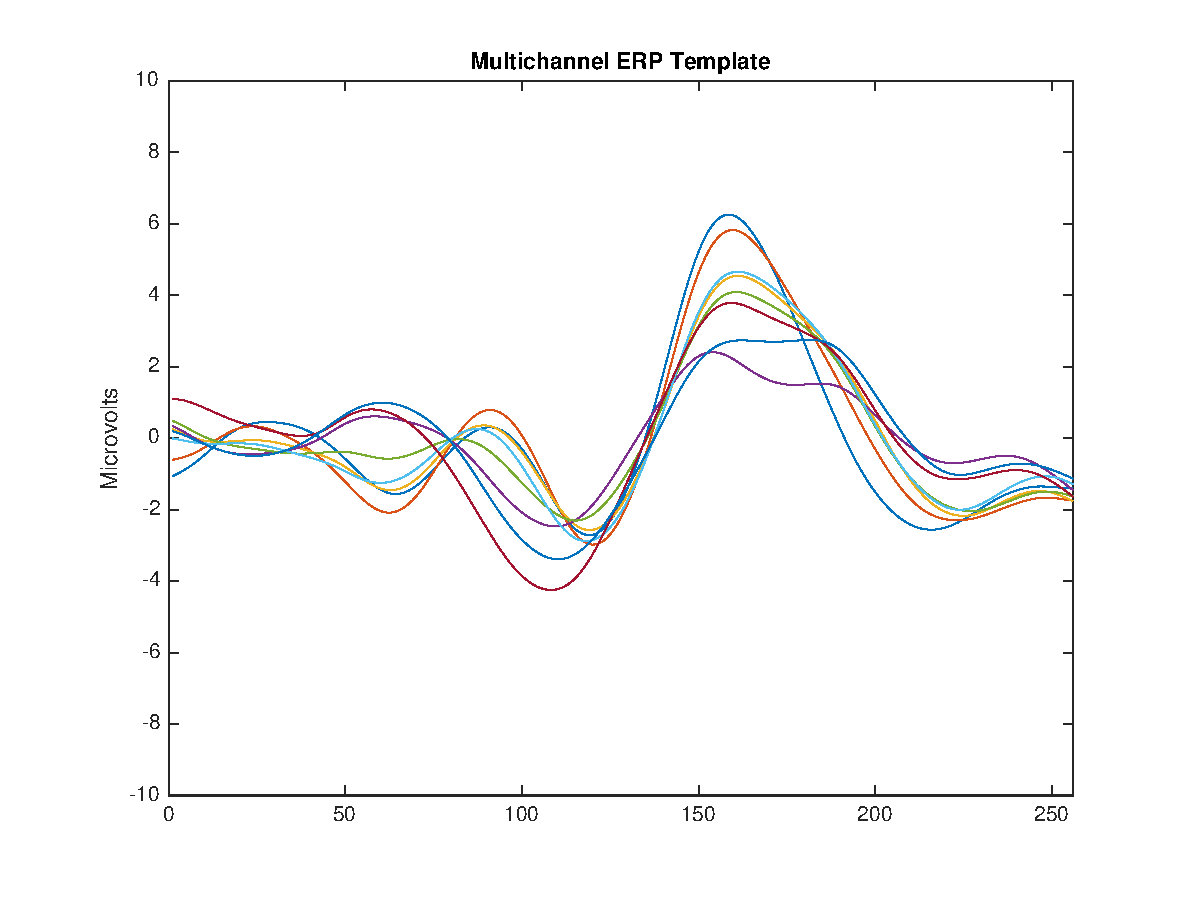
\includegraphics[width=12cm]{images/erptemplate1.eps}
\caption[P300 ERP Template]{ERP Template obtained from the coherent point-to-point ensemble average from the signals of Subject Number 8 of the Dataset I of ALS patients. The template is $1$-second long which is 256 sample points, and the eight channels are superimposed with different colors.  Vertical axis represents amplitude in $\mu V$ while horizontal axis reflects discrete sample points. The P3b component can be seen around the sample index $150$ and $200$.}
\label{fig:erptemplate1}
\end{figure}

The EEG stream with null-P300 signal is obtained by the following procedure: 
A subject participant is recruited voluntarily and the experiment is conducted anonymously in accordance with the Declaration of Helsinki published by the World Health Organization.  No monetary compensation is handed out and she/he agrees and signs a written informed consent.  This study is approved by the \textit{Departamento de Investigación y Doctorado, Instituto Tecnológico de Buenos Aires (ITBA)}.  The participant is healthy and have normal or corrected-to-normal vision and no history of neurological disorders. This voluntary subject is aged between 20-30 years old.  EEG data is collected in a single recording session. She/He is seated in a comfortable chair, with her/his vision aligned to a computer screen located one meter in front of her/him.  The handling and processing of the data and stimuli is conducted by the OpenVibe platform~\cite{Renard2010}.  Gel-based active electrodes (g.LADYbird, g.Tec, Austria) are used on locations Fz, Cz, Pz, Oz, P3,P4, PO7 and PO8 according to the 10-20 international system.  Reference is set to the right ear lobe and ground is preset as the AFz position.   Sampling frequency is set to 250 Hz.

The participant is instructed to passively watch the flashing screen while not focusing on any particular letter.  The experimental conditions are the same as those described for previous datasets.  A questionnaire is handed out at the end of the experiment with questions about how the participant felt during it, without giving more details.  

%This P300 Speller protocol consist in the flashing of 35 trails of 35 letters (7 words of 5 letter) where the intensification sequence of 6 rows and 6 columns is repeated 10 times for each letter.  More details can be found on the published work of \cite{Riccio2013}.

Figure~\ref{fig:gains} shows a $5s$ sample of the EEG trace obtained with the MNE library~\cite{Gramfort2013}.  Channel $S$ represents the twelve different stimulus markers (columns or rows) while channel $L$ represent the label (\textit{True} vs \textit{False}).  Labels are represented by square signals.  \textit{False} segments are marked with single amplitude square signals while \textit{True} segments are identified by double-amplitude square signals.  Subfigure (a) shows the signals before the ERP template is superimposed while subfigure (b) shows the same signals with the superimposed ERP template.  At first-sight, differences are really hard to spot visually.  Subfigures (c) and (d) show only one second of channels Cz and L from the same segment.  The superimposed ERP can be devised enclosed by the vertical bars, around $31.5$~$\si{seconds}$, where in (d) the peak is slightly bigger.  Figure~\ref{fig:gaincheck} shows the obtained ensemble average ERPs as result of superimposing the template signal into the EEG stream, time-locked to the stimulus onset.   These 12 point-to-point averaged segments correspond to the first trial of the EEG stream.

%The original signal-to-noise ratio was calculated as Hue 2010.

\begin{figure}[h!]
\centering
\subfigure[EEG trace of the original signal.]{\includegraphics[width=.45\linewidth]{images/nogain.eps}}
\subfigure[The same eight-channel signal segment with the superimposed template.]{\includegraphics[width=.45\linewidth]{images/singlegain.eps}}
\subfigure[EEG sample of Cz and L channel of the original EEG trace.]{\includegraphics[width=.45\linewidth]{images/nogainzoomhit.eps}}
\subfigure[The same segment with the superimposed template.]{\includegraphics[width=.45\linewidth]{images/singlegainzoomhit.eps}}
\caption[Pseudo-real Dataset EEG Streams]{Eight-channel EEG signal without and with the superimposed ERP Template. The channel L, the mark which identifies where to superimpose the P300 ERP, is shown as well as the channel S which identifies the stimulus that was presented. On (c) and (d) the small variation that was introduced by the superimposition of the ERP can be seen enclosed by the vertical bars, where the slope of the bump on subfigure (d) is slightly bigger}
\label{fig:gains}
\end{figure}

Inter- and Intra-trial variability, with eventually cognitive implications, can alter the shape of the evoked P300 potential.  Hence, it is of interest to assess  at which extend waveform-based algorithm can handle these variations. Using this dataset, the following experiments are conducted to simulate known alterations over waveform components and to verify the performance of the algorithms expounded on Section~\ref{waveformalgorithms}, \textit{MP1}, \textit{MP2}, \textit{PE}, \textit{SHCC} and the one proposed by this Thesis: \textit{HIST}.

\begin{itemize}
\item Experiment 1 - Letter Identification Performance: the letter identification performance of each one of these methods on the artificially generated pseudo-real dataset.
\item Experiment 2 - Latency Noise:  Instead of superimposing the P300 ERP over the EEG trace at the exact locations where stimulus onsets are situated, an artificial latency lag is added.  The lagging value is picked from a uniform distribution $U(0,0.4)$ [s] ranging from $0$ to $0.4$ of the $1s$ segment size~\cite{DaPelo2018}.
\item Experiment 3 - Component Amplitude Noise: the amplitude of the main P3b component of the ERP template is randomly altered.  This component is defined to be located from the stimulus onset between $148$ ms up to $996$ ms which is around $840$ ms long.  This waveform element, multiplied by a gain factor, is subtracted from the original template.  This gain factor between $0$ and $1$ is drawn from a uniform distribution $U(0,1)$.  Additionally this subtracted waveform is multiplied by a Gaussian window with a support of the same length~\cite{Harris1978}.  This avoids adding any discontinuity into the artificial generated signal.
\end{itemize}


\begin{figure}[h!]
\centering
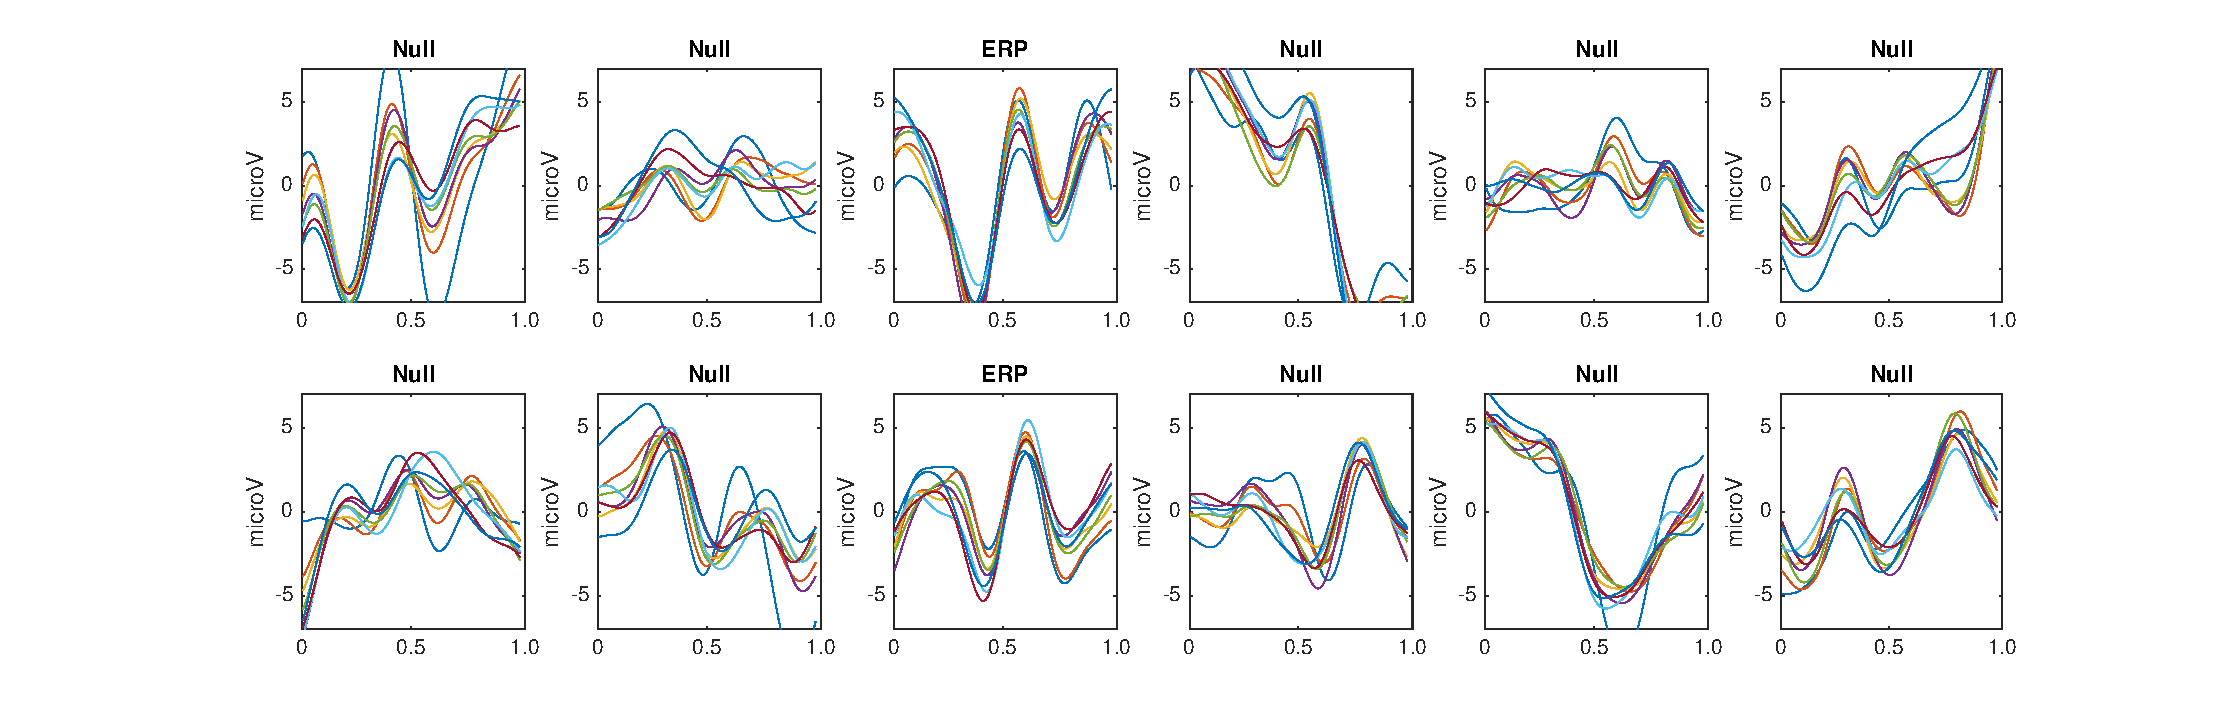
\includegraphics[width=1.0\linewidth]{images/GainCheck.eps}
\caption[P300 Averaged Segments for a single-intensification sequence]{Point-to-point averaged signals for the first letter identification trial.  The ERP is superimposed on locations 3 and 9.  Location $l=3$ is obtained while averaging the segments where the row of the speller matrix is intensified whereas locations 9 is calculated from the intensification of the corresponding column.}
\label{fig:gaincheck}
\end{figure}

The classification method Support Vector Machine \textit{SVM} with a linear kernel, is added for comparison as control using a feature $f$ constructed by normalizing the signal on each channel~\cite{Krusienski2006}.  This method has been proved efficient in decoding P300 in several BCI Competitions~\cite{Kaper2004}. 

All these experiments are executed using a cross-validation procedure dividing the letter to spell in two sets, preserving the structure of the letter identification trials. Spelling letters are scrambled while the order and group of each intensification sequence is preserved.

\subsubsection{Dataset IV - P300 Dataset IIb BCI Competition II (2003)}

Finally the performance at letter identifications for the method proposed on this Thesis and the other similar methods described in~\ref{waveformalgorithms} is evaluated by performing an offline BCI Simulation on the Dataset IIb of the BCI Competition II (2003)~\cite{Blankertz2002}.  The protocol of this dataset is very similar to what was used to obtain the pseudo-real dataset.  The sampling frequency of this dataset is $240$, the number of letters are $73$ where the first $42$ are used to create the template dictionary for all the methods and the remaining $31$ are used to test the character recognition rate performance.  

%TODO Explicar este protocolo porque no es igual, de hecho es bastante distinto.

\subsubsection{Parameters}

The P300 event can have a span $\gls{lambda}$ of $400$ ms and its peak-to-peak amplitude $\gls{DeltamuV}$ can reach $ 10 \mu V $~\cite{Rao2013}.  Hence it is necessary to utilize a signal segment of size $\gls{w} = 1$ second.  In order to compute the patch parameters, Equations~\ref{eq:horizontalpatchscale} and \ref{eq:verticalpatchscale} are used to determine the value of $3$ for the horizontal patch scale $\gls{St}$ as well as the vertical patch scale $\gls{Sv}$.  It is important to remark that as it is described in Section~\ref{Pipeline} the effective sampling frequency $\gls{Fs}$ of the signal is $16$~$\si{\hertz}$.


%necesitamos definir el valor de s en función de los parámetros de la señal, de modo tal que el parche cubra el evento completo.  
%We propose the Equations~\ref{eq:mapping2} and~\ref{eq:mapping1} to compute the scale value in horizontal and vertical directions, respectively. 
%\begin{equation}
%s_x = \frac{ \gamma \;  \lambda \  F_s}{12}
%\label{eq:mapping2}
%\end{equation}
%
%\begin{equation}
%s_y= \frac{\gamma \; \Delta \mu V}{12} 
%\label{eq:mapping1}
%\end{equation}

As the peak-to-peak amplitude is small, to have a better resolution, the amplitude scales parameter are selected to be  $ \gamma = 4 $, and $\gls{gammat} = 4$.  With this configuration, the local patch and the descriptor can identify events of at most 16 $ \mu V $ of amplitude, with a span of $ \lambda = 0.99$ seconds, covering almost the entire segment.  According to Equations~\ref{eq:resolutiony} and \ref{eq:resolutionx}, this also determines that $ 1 $ pixel represents $ \frac{1}{\gamma}= \frac{1}{4} \mu V $ on the vertical direction, and $\frac{1}{\gls{Fs} \ \gls{gammat} }=\frac{1}{64}$ seconds on the horizontal direction. The keypoints  $\gls{kp}$  are located at $ (x_{k_p}, y_{k_p} )= ( 0.55 \gls{Fs} \ \gls{gammat}, z^l(c) )= (35,  z^l(c)) $ for the corresponding channel $c$ and location $l$ (see Equation~\ref{eq:zerolevel}).   In this way the whole transient event is captured. 

Lastly, the number of channels $\gls{C}$ is equal to $8$ for the first three datasets and the number of intensification sequences $\gls{ka}$ is fixed to $10$, whereas for the Dataset IV of the BCI Competition, $\gls{C}$ is equal to $64$ and the value $\gls{ka}$ is equal to $15$.   The parameter $\gls{k}$ used to construct the set $N_T(\mathbf{q}^{(l,c)})$ is assigned to $k=7$, which was found empirically to achieve better results.  In addition, the norm used on  Equations \ref{eq:multiclassificationrow} and \ref{eq:multiclassificationcol} is the cosine norm, and descriptors are normalized to $ \left[ -1, 1 \right] $ (check Chapter~\ref{chapter:eleven}).

\section{Results}

Table~\ref{tab:resultsals} shows the results of applying the Histogram of Gradient Orientations (HIST) algorithm to the subjects of the Dataset I of ALS patients. The percentage of correctly spelled letters is calculated while performing an offline BCI Simulation.  From the seven words for each subject, the first three are used for calibration, and the remaining four are used for testing.  The best performing channel  $\gls{bpc}$ is informed as well. The target ratio is $1:36$; hence theoretical chance level is $2.8\%$. It can be observed that the best performance of the letter identification method is reached in a dissimilar channel depending on the subject being studied.  Moreover, this table shows for comparison the obtained performance rates using single-channel signals with the Support Vector Machine (SVM) classifier.  This method is configured to use a linear kernel.  The best performing channel $\gls{bpc}$, where the best letter identification rate was achieved, is also depicted.


\begin{table}[h!]
\caption[Dataset I - Single Channel Character Recognition Rates]{Dataset I: Character recognition rates for the public dataset of ALS patients using HIST calculated from single-channel plots.  Performance rates using single-channel signals with the SVM classifier are shown for comparison.  The best performing channel $bpc$ for each method is visualized}
\centering
%% \tablesize{} %% You can specify the fontsize here, e.g.  \tablesize{\footnotesize}. If commented out \small will be used.
\begin{tabular}{c|cc|cc}
\toprule
\textbf{Participant}	&  $bpc$ 	&  HIST &  $bpc$	&  Single Channel SVM \\
\midrule
1     &     Cz   &   $35\%$    &  Cz   & $15\%$   \\
2     &     Fz   &   $85\%$      &  PO8   & $25\%$   \\
3     &     Cz   &   $25\%$    &  Fz   & $5\%$   \\
4     &     PO8 &   $55\%$   &  Oz   & $5\%$    \\
5     &     PO7 &   $40\%$    &  P3   & $25\%$   \\
6     &     PO7 &   $60\%$  &  PO8   & $20\%$    \\
7     &     PO8 &   $80\%$   &  Fz   & $30\%$     \\
8     &     PO7 &   $95\%$     &  PO7   & $85\%$ \\

%\bottomrule
\end{tabular}
\label{tab:resultsals}
\end{table}

%The spelled words are \textit{MANSO},\textit{CINCO},\textit{JUEGO} and \textit{QUESO}.

\begin{figure}[h!]
\centering
\includegraphics[width=10cm]{images/performance.eps}
\caption[Dataset I ALS Patients Dataset P300 Performance Curves]{Performance curves for the eight subjects included in the dataset I of ALS patients.  Three out of eight subjects achieved the necessary performance to implement a valid P300 speller.}
\label{fig:performance}
\end{figure}

% Agregar la clasificacion perfecta en base a que no considerabamos la varianza de la senial graficada

%The spelled words are \textit{GATTO}, \textit{MENTE}, \textit{VIOLA} and \textit{REBUS}.

The Information Transfer Rate (ITR), or Bit Transfer Rate (BTR), in the case of reactive BCIs~\cite{WolpawJonathanR2012}  depends on the amount of signal averaging required to transmit a valid and robust selection.  Figure~\ref{fig:performance} shows the performance curves for varying intensification sequences for the subjects included in the dataset of ALS patients. It can be noticed that the percentage of correctly identified letters depends on the number of intensification sequences that are used to obtain the averaged signal.  Moreover, when the number of intensification sequences tend to 1, which corresponds to single-intensification character recognition, the performance is reduced. As mentioned before, the SNR of the P300 obtained from only one segment of the intensification sequence is very low and the shape of its P300 component is not very well defined.

\begin{table}[h!]
\caption[Dataset II - Single Channel Character Recognition Rates]{Dataset II: Character recognition rates and $bpc$  using HIST calculated from  single-channel signals.  Performance rates using single-channel signals with the SVM classifier are shown for comparison.}
\centering
%% \tablesize{} %% You can specify the fontsize here, e.g.  \tablesize{\footnotesize}. If commented out \small will be used.
\begin{tabular}{c|cc|cc}
\toprule
\textbf{Participant}	&  $bpc$	&  HIST &  $bpc$	&  Single Channel SVM \\
\midrule
1     &     Oz   &   $40\%$  &  Cz   &  $10\%$    \\
2     &     PO7   &   $30\%$      &  Cz   & $5\%$   \\
3     &     P4   &   $40\%$    &  P3   & $10\%$    \\
4     &     P4 &   $45\%$    &  P4   & $35\%$     \\
5     &     P4 &   $60\%$  &  P3   & $10\%$     \\
6     &     Pz &   $50\%$ &  P4   & $25\%$     \\
7     &     PO7 &   $70\%$  &  P3   & $30\%$     \\
8     &     P4 &   $50\%$    &  PO7   & $10\%$    \\

%\bottomrule
\end{tabular}
\label{tab:resultsown}
\end{table}


In Table~\ref{tab:resultsown} the results obtained for 8 healthy subjects are shown.  It can be observed that the performance is above chance level. It was verified that HIST method has an improved performance at letter identification than SVM that process the signals on a channel by channel strategy (Wilcoxon signed-rank test, $p =  0.004$ for both datasets).


\begin{table}[h!]
\caption[Dataset I - Comparisons of Character Recognition Rates]{Character recognition rates and the best performing channel $bpc$ for the public dataset I  using the HIST versus performance rates obtained by SWLDA and SVM classification algorithms with a multichannel concatenated feature.}
\centering
%% \tablesize{} %% You can specify the fontsize here, e.g.  \tablesize{\footnotesize}. If commented out \small will be used.
\begin{tabular}{c|cc|c|c}
\toprule
%\textbf{Participant}	&  \textbf{BPC}	& \multicolumn{2}{c}{Character Recognition Rates}\\
%\cline{1-5} \\
\textbf{Participant}	&  $bpc$	&  HIST & Multichannel SWLDA & Multichannel SVM \\
                                    &  for HIST        &           &                                       &   \\
\midrule
1     &     Cz   &   $35\%$  & $45\%$  & $40\%$\\
2     &     Fz   &   $85\%$  & $30\%$   & $50\%$   \\
3     &     Cz   &   $25\%$  & $65\%$ & $55\%$   \\
4     &     PO8 &   $55\%$ & $40\%$  & $50\%$   \\
5     &     PO7 &   $40\%$ & $35\%$  & $45\%$   \\
6     &     PO7 &   $60\%$ &  $35\%$  & $70\%$   \\
7     &     PO8 &   $80\%$ & $60\%$   & $35\%$   \\
8     &     PO7 &   $95\%$  & $90\%$   & $95\%$  \\

%\bottomrule
\end{tabular}
\label{tab:resultsalsswlda}
\end{table}

%In Tables~\ref{tab:resultsals} and~\ref{tab:resultsown} results for character recognition rates using single channel signals with the SVM~\cite{Scholkopf2001}  classification algorithm are also shown.    This algorithm was configured to use a linear kernel.  The best performing channel where the best letter identification rate was obtained is also depicted.

%The PE algorithm, which is also devised on a time-domain description of the waveform, was implemented according to \cite{Unakafova2013} and its parameters were adjusted as stated by \cite{Zanin2012}, with an \textit{order} of $2$ and a \textit{sliding window} of size $10$. 

Tables~\ref{tab:resultsalsswlda} and~\ref{tab:resultsownswlda} are presented in order to compare the performance of the HIST method versus a multichannel version of the SWLDA and SVM classification algorithms for both datasets.  The feature was formed by concatenating all the channels~\cite{Krusienski2006}.  SWLDA is the methodology proposed by the ALS dataset's publisher.  As can be observed in Figure~\ref{fig:boxplots}, it was verified for the dataset I of ALS patients that HIST has similar performance  against other methods like SWLDA or SVM, which use a multichannel feature (Quade test with $p=0.55$) whereas for the dataset of healthy subjects significant differences were found (Quade test with $p=0.02$) where only the HIST method achieved a different performance than SVM (with multiple comparisons, significant difference of level $0.05$).

\begin{figure}[h!]
\centering
\includegraphics[width=10cm]{images/boxplots.png}
\caption[Dataset I and II Performances Boxplots]{Boxplots obtained for the methods HIST and multichannel SVM and SWLDA for the Datsets I and II.  The achieved performance for the HIST method is similar to the performace obtained for the other methods (Quade test with $p=0.55$).}
\label{fig:boxplots}
\end{figure}

\begin{table}[h!]
\caption[Dataset II - Comparisons of Character Recognition Rates]{Character recognition rates and the best performing channel $bpc$ for the  dataset II  using HIST versus performance rates obtained by SWLDA and SVM classification algorithms with a multichannel concatenated feature.}
\centering
%% \tablesize{} %% You can specify the fontsize here, e.g.  \tablesize{\footnotesize}. If commented out \small will be used.
\begin{tabular}{c|cc|c|c}
\toprule
%\textbf{Participant}	&  \textbf{BPC}	& \multicolumn{2}{c}{Character Recognition Rates}\\
%\cline{1-5} \\
\textbf{Participant}	&  $bpc$ 	&  HIST & Multichannel SWLDA & Multichannel SVM  \\
                                    &  for HIST        &           &                                       &   \\
\midrule
1     &     Oz   &     $40\%$  &     $65\%$  &     $40\%$ \\
2     &     PO7   &     $30\%$ &   $15\%$  &     $10\%$ \\
3     &     P4   &     $40\%$ &     $50\%$  &     $25\%$ \\
4     &     P4   &     $45\%$ &     $40\%$  &     $20\%$ \\
5     &     P4   &      $60\%$ &    $30\%$  &     $20\%$ \\
6     &     Pz   &      $50\%$ &    $35\%$  &     $30\%$ \\
7     &     PO7   &      $70\%$ &  $25\%$  &     $30\%$ \\
8     &     P4   &      $50\%$ &    $35\%$  &     $20\%$ \\

%\bottomrule
\end{tabular}
\label{tab:resultsownswlda}
\end{table}

%It was verified for the dataset of ALS patients that it has similar performance  against other methods like SWLDA or SVM, which use a multichannel feature (Quade test with $p=0.55$) whereas for the dataset of healthy subjects significant differences where found (Quade test with $p=0.02$) where the HIST method achieved a better performance than SVM (with multiple comparisons, significant difference of level $0.05$).
 
%\subsection{Occipital Channels}

The P300 ERP  consists of two overlapping components: the P3a and P3b, the former with frontocentral distribution while the later stronger on centroparietal region~\cite{Polich2007}. Hence, it is known that the stronger response of this ERP is usually found on the central channel Cz~\cite{Riccio2013}. However, \cite{Krusienski2006} shows that the response may also arise in occipital regions.  We found that by analyzing only the waveforms, occipital channels PO8 and PO7 show higher performances for some subjects. 

%\subsection{Stability of the P300 shape}

As subjects have varying \textit{latencies} and \textit{amplitudes} of their P300 components, they also have a varying stability of the \textit{shape} of the generated ERP \cite{Nam2010}.  Figure~\ref{fig:p300templates} shows 10 sample P300 templates patches for patients 8 and 3 from the Dataset I of ALS patients. It can be discerned that in coincidence with the performance results, the P300 signature is more clear and consistent for subject 8 (A) while for subject 3 (B) the characteristic pattern is more difficult to perceive.


\begin{figure}[h!]
\centering
\includegraphics[width=15cm]{images/subject.png}\label{subject8}
\caption[Sample P300 Patches]{Ten sample P300 template patches for Subjects 8 (A) and 3 (B) of the public Dataset I of ALS patients.}  %Downward deflection is positive polarity. 
\label{fig:p300templates}
\end{figure}


Additionally, the stability of the P300 component waveform has been extensively studied in patients with ALS \cite{SellersandEmanuelDonchin2006,TomohiroMadarame2008,Nijboer2009,Mak2012,McCane2015} where it was found that these patients have a stable P300 component, which were also sustained across different sessions.  In line with these results we do not find evidence of a difference in terms of the performance obtained by analyzing the waveforms, by using the HIST method, for the group of patients with ALS and the healthy group of volunteers (Mann-Whitney U Test, $p=0.46$). Particularly, the best performance is obtained for a subject from the ALS dataset for which, based on visual observation, the shape of they P300 component is consistently identified.

%\subsection{Descriptor Space and classification method}

It is important to remark that when applied to binary images obtained from signal plots, the feature extraction method described in Section \ref{SIFT} generates sparse descriptors.  Under this subspace we found that using the cosine metric yielded a significant performance improvement (check Chapter~\ref{chapter:eleven}). On the other hand, the unary classification scheme based on the NBNN algorithm proved very beneficial for the P300 Speller Matrix.  This is due to the fact that this approach solves the unbalance dataset problem which is inherent to the oddball paradigm~\cite{Tibon2015}.  

%Using the same feature but with classification methods SVM, feed forward Neural Networks and SWLDA  common in BCI Research achieved a reduced performance.


Regarding Experiments 1, 2 and 3 for the Dataset III, results are shown in Table~\ref{tab:results} and in Figure~\ref{fig:performancetest}, ~\ref{fig:performancetestlatency} and~\ref{fig:performancetestamplitude}.  Table~\ref{tab:results} shows the  performance for the Experiment I, II and III while identifying each letter of the standard P300 Speller Matrix, and the $\gls{bpc}$, the channel where the best performance is attained.   Figure~\ref{fig:performancetest} shows the performance curves attained for the Experiment 1, for the six algorithms under comparison.  Each one represents the percentage of letters that is actually predicted by each algorithm using a cross-validation procedure.  As previously described the data is continuously divided in two sets, where the first 15 letters are used to derive the dictionary of templates while the remaining 20 letters are used to measure the letter identification performance. This is repeated one hundred times, and performances averaged.   Figure~\ref{fig:performancetestlatency} shows the same results for the Experiment 2, where a noisy latency lag was included.   Last but not least, Figure ~\ref{fig:performancetestamplitude} represents the performance values obtained for the Experiment 3, when the amplitude of the P3b component of the template is randomly attenuated.  

A significant reduction of performance was found when latency noise is added (Experiment 1 vs 2, Wilcoxon rank sum test, one tail, with $p=0.0022$).  The latency noise added to each segment $S_i^l$ under the Experiment 3, reduces the information contained in the averaged signal, mainly due to the invalidation of the SNR enhancement performed by the signal averaging procedure.  This reduction alters the obtained shape of the waveform of the ERP and impacts on the performances regardless of the method. On the other hand, all the algorithms show some resistance to noise in peak amplitudes of the main component. This is shown by the similarities of obtained results between the Experiment 1 and 3 (Wilcoxon rank sum test, two tails, not rejected with $p=0.1797$).  Additionally, a two-way balanced Quade test was performed to evaluate the performance's differences for the three experiments for the dataset III, and for the six methods.  Difference among the method's letter identification rates were found with $p=0.0019$.  The methods \textit{SHCC}, \textit{HIST}, \textit{MP-1} performed much better than the other algorithms, including \textit{SVM}.  By making multiple comparisons at a level  $0.05$, significant differences are found between \textit{SHCC} vs MP-1,MP-2, PE and SVM, between \textit{HIST} vs. MP-2 and PE, and between \textit{SVM} and MP-2.

\begin{figure}[h!]
\centering
\includegraphics[width=15cm]{images/CrossPerformanceTest.eps}
\caption[Experiment I Pseudo-real Dataset III Speller Performance]{Speller performance obtained for each method for the Experiment 1.  Y-axis shows performance accuracy while X-axis shows the number of intensification sequences used to calculate the point-to-point signal average.}
\label{fig:performancetest}
\end{figure}

\begin{figure}[h!]
\centering
\includegraphics[width=15cm]{images/CrossPerformanceTestLatency.eps}
\caption[Experiment II Pseudo-real Dataset III Speller Performance]{Speller performance obtained for each method while latencies are artificially added to each single-intensification segment corresponding to the Experiment 2.  The achieved performance is significantly reduced for all methods. Y-axis shows letter identification performance while X-axis shows the number of intensification sequences used to calculate the ensemble average.}
\label{fig:performancetestlatency}
\end{figure}

\begin{figure}[h!]
\centering
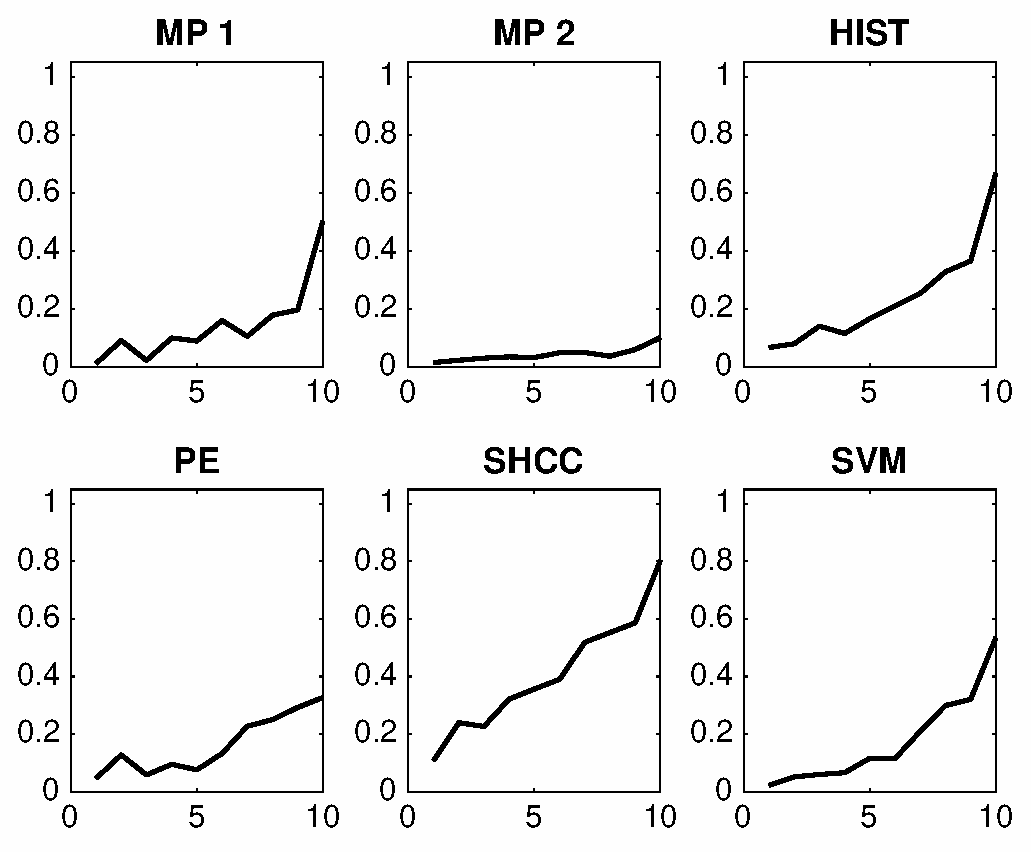
\includegraphics[width=15cm]{images/CrossPerformanceTestAmplitude.eps}
\caption[Experiment III Pseudo-real Dataset III Speller Performance]{Speller performance obtained for the Experiment 3 while the amplitudes of the P3b component of the superimposed ERP are randomly reduced. Y-axis shows performances for character recognition rates while X-axis shows the number of intensification sequences.}
\label{fig:performancetestamplitude}
\end{figure}

\begin{table}[h!]
\caption[Pseudo-real Dataset Speller Performance]{Speller classification performance obtained for all the waveform-based algorithms: MP Matching Pursuit, HIST Histogram of Gradient Orientation, PE Permutation Entropy and SHCC Slope Horizontal Code Chain. Additionally, the control algorithm SVM Support Vector Machines is included for comparison.  All the methods process the signal on a channel-by-channel basis, hence the best performing channel is also shown. In this case with absence of null-signals, it can be interpreted as the channel that adds less noise to the ERP template.  All the methods used $10$ intensification sequences to coherently average the trials to obtain the averaged signal. }
\centering
%% \tablesize{} %% You can specify the fontsize here, e.g.  \tablesize{\footnotesize}. If commented out \small will be used.
\begin{tabular}{ccccc}
\toprule
\textbf{Method}	& \textbf{$\gls{bpc}$} &   \multicolumn{3}{c}{Performance} \\
%\cline{3-5} \\
 	&  &  \textbf{Experiment 1} & \textbf{Experiment 2}	& \textbf{Experiment 3}\\
\midrule
MP 1 & PO8  & $67\%$ & $15\%$ & $50\%$\\
MP 2 & PO7 & $24\%$ & $6\%$ & $10\%$\\
HIST  & PO8 & $91\%$ & $18\%$ & $66\%$\\
PE     & Cz & $61\%$ & $9\%$ & $32\%$\\
SHCC & P4 & $98\%$ & $31\%$ & $80\%$\\
SVM     & PO8  & $78\%$ & $7\%$ & $53\%$\\
\bottomrule
\end{tabular}
\label{tab:results}
\end{table}

Finally, results obtained for the dataset BCI Competition 2003 IIb are shown in Figures \ref{fig:performancebcicompetition} and in Table~\ref{tab:bcicompetitionresults}.  As mentioned before, for this experiment the number of available intensification sequences is $15$. The obtained character identification rate is above theoretical chance level, and for HIST close to the usable threshold of $70\%$~\cite{Kathner2017}.

\begin{table}[h!]
\caption[Dataset IIb BCI Competition II (2003) Speller Performance]{Speller classification performance obtained for Dataset IV, the dataset IIb of the BCI Competition II (2003), for each one of the algorithms using $15$ repetitions of intensification sequences. The first $42$ trials are used for training to build the template dictionary and the remaining $31$ for testing. The channel where the best performance is attained, is also shown. }
\centering
%% \tablesize{} %% You can specify the fontsize here, e.g.  \tablesize{\footnotesize}. If commented out \small will be used.
\begin{tabular}{ccc}
\toprule
\textbf{Method}	& \textbf{$\gls{bpc}$} &  \textbf{Performance} \\
\midrule
MP 1 & FC2  & $50\%$ \\
MP 2 & CPz & $22\%$ \\
HIST  & Cz & $67\%$ \\
PE     & PO8 & $22\%$ \\
SHCC & Cz & $61\%$ \\
SVM     & C1  & $32\%$ \\
\bottomrule
\end{tabular}
\label{tab:bcicompetitionresults}
\end{table}

\begin{figure}[h!]
\centering
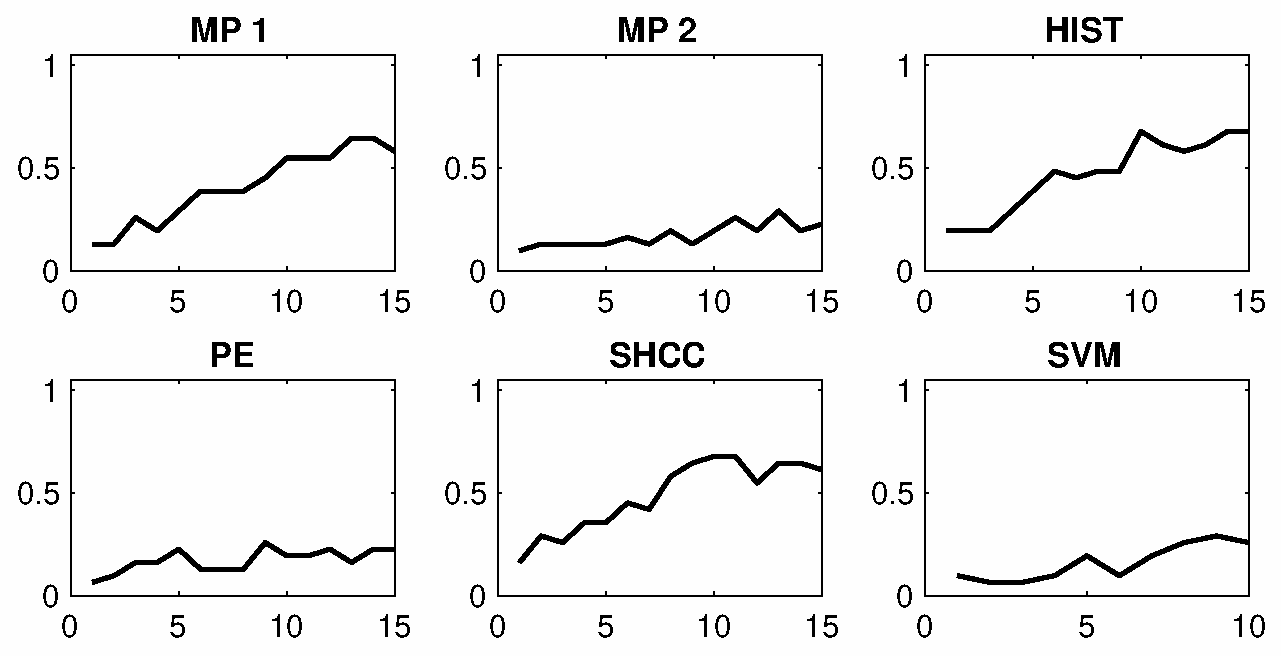
\includegraphics[width=15cm]{images/PerformanceBCICompetition.eps}
\caption[Dataset IIb BCI Competition II (2003) Speller Performance]{Speller performance obtained for the Dataset IV (Dataset IIb of the BCI Competition II 2003) for each one of the algorithms.  An offline BCI Simulation is performed using the first $42$ trials as training and the remaining $31$ as testing.  The horizontal axis show the number of intensification sequences, from $0$ to $15$ for this dataset, while the vertical axis show the performance rate.}
\label{fig:performancebcicompetition}
\end{figure}

\section{Conclusion}

%In this paper, a new unsupervised method to enhance evoked response by target stimuli in an oddball paradigm was presented. Only given the time indexes of rows/columns intensifications, the proposed algorithm estimates the main components of the P300 subspace by providing the best SNR. It was shown to efficiently improve the quality of the evoked responses by taking into account the signal and the noise, as opposed to principal component analysis, which only considers the signal. Using this method to enhance P300 subspace before the BCI classification task speeds up the BCI since less words are required to train the spatial filters and the linear classifier, given a certain percentage of good symbol prediction. Moreover, using this spatial enhancement significantly reduces the dimension of the feature vector used to predict words.

%For both datasets, the experimental protocol uses a very short inter-stimulus interval which has the potential to increase the ITR but at the same time it reduces the amplitude of the P300 response, hence it may be more difficult to detect it~\cite{Rao2013}.   It is known that ISI alters the P300 amplitude and may affect the chance to detect the ERP.

%In the case of the P300 response, the oddball paradigm requires that one of the stimuli be infrequent. Hence this forces the data to be unbalanced~\cite{Tibon2015}.  At the same time, the NBNN method suffers from biased classification on unbalanced classes~\cite{Fornoni2014}. %Para solucionar este problema, 

The usage of the Histogram of Gradient Orientations to implement a valid P300-Based BCI Speller application is expounded.  Additionally, its validity is, first, evaluated using a public dataset of ALS patients and an own dataset of healthy subjects.  Second, the method is contrasted against other approaches based on a shared similar idea and results are presented.  Finally, the method is used on a public dataset of a BCI Competition.

%The method works on a channel by channel basis; in this way the best performing channel can be identified and used it to reduce the number of required EEG electrodes, leading to the development of more ergonomic capturing device.

It is verified that HIST has an improved performance at letter identification than other methods that process the signals on a channel by channel strategy, and it even has a comparable performance against other methods like SWLDA or SVM, which uses a multichannel feature.
Furthermore, this method has the advantage that shapes of waveforms can be analyzed in an objective way.  We observed that the shape of the P300 component is more stable in occipital channels, where the performance for identifying letters is higher.   We additionally verified that ALS P300 signatures are stable in comparison to those of healthy subjects.

%Further work should be conducted over larger samples to cross-check the validity of these results.

We believe that the use of descriptors based on the histogram of gradient orientation, presented in this work, can also be utilized for deriving a shape metric in the space of the P300 signals which can complement other metrics based on time-domain as those defined by~\cite{Mak2012}. It is important to notice that the analysis of these waveform shapes is usually performed in a qualitative approach based on visual inspection~\cite{SellersandEmanuelDonchin2006}, and a complementary methodology which offer a quantitative metric will be beneficial to these routinely analysis of the waveform of ERPs.

%and, based on this idea, we wanted to complement the methodology with a cuantitative and objective sight

Considering other methods inspired on the same idea, we verified that similar performance results are obtained for the methods \textit{SHCC}, \textit{HIST} and \textit{MP-1} and that it is also possible to obtain discriminating information from the underlying signal based exclusively on an automated method of processing the waveforms.  

The goal of this Chapter is to answer the question if a P300 component could be solely determined by inspecting automatically their waveforms.  We conclude affirmatively, though two very important issues still remain:

First, a correct alignment of the segments used on the averaging procedure is crucial: a preliminary approach was tested to assess if the waveform shape of the P300 of the averaged signal can be improved (i.e. more visually similar between different trials) by applying different alignments of the stacked segments (see Figure~\ref{fig:classification}) and it was verified that there is a better performance when a correct segment alignment regularize the averaged waveform.  We applied Dynamic Time Warping (DTW)~\cite{Casarotto2005} to automate the alignment procedure but we were unable to find a substantial improvement.  Further work to study the alignment of segments on averaging procedures,  should be addressed.

The second problem is the amplitude variation of the P300.  Standardizing the averaged signal, as described in Equation~\ref{eq:standarizedaverages} has the effect of normalizing the peak-to-peak amplitude, moderating its variation. It has also the advantage of reducing noise that was not reduced by the averaging procedure.   It is important to remark that the averaged signal variance depends on the number of segments used to compute it \cite{van2006signal}.  The standardizing process converts the variance of this averaged signal to unit variance which makes it independent of the number segments used to compute the average.   Although this is initially an advantageous approach, this standardizing process also reduces the amplitude of any significant P300 complex wave, diminishing its automatic interpretation capability.


%The spelled words are \textit{GATTO}, \textit{MENTE}, \textit{VIOLA} and \textit{REBUS}.

%The purpose of this work is threefold, (1) raise awareness about the utility of using automatic waveform-based methods to study EEG signals, (2) to provide an overview of the state-of-the-art of those methods, and (3) to compare those methods and verify if it is possible to obtain acceptable classification performances based exclusively on the signal's waveform.

%\chapter{Epilogue}
\label{chapter:seven}

%This thesis humbly offers a method and framework to study EEG brain signal waveforms.  

In the first Chapter, the following question was posed:  is it possible to analyze and discriminate electroencephalographic signals by automatic processing the shape of the waveforms using the Histogram of Gradient Orientations ? \\ 

%Que es diferente en mundo de EEG y BCI a partir de esta tesis?
%lo que es diferente es que se puede implementar un metodo que toma una metrica objetiva de la forma de la se;al antes no existia bien
%esta tesis fomenta esa conexion, que puede ser provechosa por facotres que se discutiran luego
%se ofrece un marco general para abordar este estudio que puede luego explotarse desde otras sdisciplinas similares.  Nos queda la sensacion de muchos cabos a futuro que explotar y esta conclusion y este capitulo justamente abordara esos temas

We conclude affirmatively, and remark the following points:

%\textbf{What is different in the world after the submission of this Thesis?}
%
%A framework and a method to analyze objectively the waveform of an EEG signal is now proposed.
%Additionally a general framework to study waveforms is proposed.  We have the feeling that there is threads to pull out of this work, and there are many areas that could be beneficed from this work and extensions.  This is the topic of this last final, and conclusive, Chapter.

\begin{itemize}
\item EEG Waveforms can be analyzed by this method.
\item Oscillatory processes can be studied by the shape of the plots.
\item The stability of ERP components can be studied objectively with the proposed method.
\end{itemize}

%The scientific or technological endeavor has been enlighten many times by the connection of initially unrelated topics.  
At the conclusion of this work, we think that there are many potential benefits from the application of this technique and that there are many areas that could be improved from this work and extensions.   
%This is the topic of this last, final, and conclusive, Chapter.

\section{Conclusions}

%Among other applications of Brain Computer Interfaces, the goal of the discipline is to provide communication assistance to people affected by neuro-degenerative diseases, who are the most likely population to benefit from BCI systems and EEG processing and analysis~\cite{WolpawJonathanR2012}.

In this Thesis, a method to analyze EEG signals based on the waveform characterization, is presented. The proposed procedure transforms the signal into an image, plots the signal on it, and analyzes their local structure using the Histogram of Gradient Orientations.   Aiming to offer a BCI implementation, this technique is adapted to perform a feature extraction procedure.  Finally a classification scheme is outlined.

This method is verified on EEG oscillatory processes.  An experiment with ten subjects and using a commercial-grade device, is conducted.  The application of the method effectively detects Alpha Waves from signals, differentiating two mental states.  It is also proved on a public dataset.  The prevalence of these signals in occipital areas is determined by a higher accuracy obtained for those brain regions.

The applicability of the method is extended to study transient signals, particularly the P300 ERP,  due to the their importance, and widespread adoption in BCI.  The method to  extract the ERP waveform is expounded and used to recognize it from EEG signals by analyzing their waveform shape.  An additional experiment on eight healthy subjects is performed but using a research-grade EEG device, specifically designed for this discipline.  The procedure is tested against the produced dataset and a usable level of accuracy, is obtained.  A BCI simulation is also implemented against a public dataset of ALS patients where it is verified that the waveform of the P300 is stable regardless of the health condition, offering an alternative method to study waveform stability.  A pseudo-real dataset is created to test for regular issues with ERP extraction procedures and the method proposed here is additionally contrasted against a set of other four alternative methods which are inspired in analyzing EEG waveforms.  It is found that this method achieved higher or equal performance values than the other methods.

%\textbf{Multichannel}
%More importantly, as with any other BCI technique, assessment on the prospects and usefulness of this procedure on the golden standard of online validation must be performed to avoid the MMLD dilemma [16].

%\begin{story}[To keep in mind]
%Among other applications of Brain Computer Interfaces, the goal of the discipline is to provide communication assistance to people affected by neuro-degenerative diseases, who are the most likely population to benefit from BCI systems and EEG processing and analysis~\cite{WolpawJonathanR2012}.
%\end{story}

\vspace{5pt}

This technique has the following benefits:

\begin{enumerate}
\item Universal applicability,
\item Objective waveform metric,
\item Foster clinical interaction,
\item Clinical-tool making,
\item Intelligible property and BCI reliability.
\end{enumerate}

\textbf{Universal applicability:}
The Histogram of Gradient Orientation method has a potential universal applicability, because the same basic methodology can be applied to detect different patterns in EEG signals with applications to BCI.   The search for meaningfull or cognitive waveforms, or \textit{cognemes} is a very important issue in BCI, neuroscience research and neurophysiology. Automatic classification of patterns in EEG that are specifically identified by their shapes like K-Complex, Vertex Waves, Positive Occipital Sharp Transient~\cite{Hartman2005} are a prospect future work to be considered. 

% Alpha waves references.

\textbf{Objective waveform metric:}
Descriptors are a direct representation of the shape of signal waveforms. Hence,  they can be used to build databases of quantitative descriptions of known waveforms and improve atlases, which are currently based on qualitative descriptions of signal shapes.

\textbf{Foster clinical collaboration:}
In our opinion, the best benefit of the presented method is that a closer collaboration of the field of BCI with physicians can be fostered, since this procedure intent to imitate human visual observation. After all analyzing waveforms by their waveform shapes is a established procedure of the clinical EEG community. One of the main goals of the BCI discipline is to provide assistance to patients and to provide alternative tools to be used in diagnostics and rehabilitation procedure.  This requires a clinical focus which is often neglected in BCI research. 

\textbf{Clinical tool-making:}
The method presented in this Thesis offers the ability to identify waveforms shapes in an exhaustive manner.  This can eventually provide assistance to physicians to localize EEG patterns, specially in long recordings periods, frequent in clinical sleep studies or neonatal ICU.  Additionally, it can be used for artifact removal which is performed on many occasions by visually inspecting signals. %Long Term recording ~\cite{Michel2012}

% \cite{Temko2016}.  SDA
%BCI Security (IEEE Paper Life Science)

\textbf{Intelligible property and BCI reliability:}
BCI reliability is yet an unfulfilled goal in this discipline~\cite{WolpawJonathanR2012}. The convenience of analyzing or including metrics about the shape of the EEG, is that clinical EEG diagnosis may support a vast set of already understood knowledge which is based on identifying EEG patterns by their shape and that can steer towards a more robust implementation of BCI devices.  

%No method will be reliable and widespread adopted until it is clear how any decision was coined. And at the same time, a method which is good enough but can be easily understood may be tide-turning in clinical acceptance.

Moreover, this conventional clinical method of observing the waveform is understood to be subjective and laborious because results depend on the technicians' experience and expertise.   At the same time, it is a subjective time-consuming task, with long-learning curves, requires specialized personnel, and it has significant error rates~\cite{Tjepkema-Cloostermans2018}.  These problems has pushed for the development of quantitative EEG, to automate the decoding of brain signals~\cite{Thakor2004}.  In spite of this, the clinical conventional practice has not been replaced and it is still widespread: the gold standard in clinical EEG is still \textit{Eye Ball}.
 %~\cite{Wulsin2011,Tjepkema-Cloostermans2018}.  

We believe that the adoption of a \textit{hybrid} methodology which can process the signal automatically, but at the same time, maintains an inherent intelligible property~\cite{j2018challenge} that can be mapped to existing procedures, and above all, can maintain the clinician trust on the system behavior, is beneficial to Clinical Practice, Neuroscience and BCI research. 

% This is an important area for future study.

%=======================================

\section{Future Work}

There are potential areas that could be improved upon the presented methodology:

\begin{enumerate}
\item Multichannel extension
\item Scale space analysis on EEG for keypoint localization
%\item Usage to determine trial to trial variability (using general orientation)
\item Neuroimaging
\item Ensemble classifiers
\item Computer vision interdisciplinary work
\item Extension to other disciplines
\end{enumerate}

\textbf{Multichannel extension:}
The methods described in section~\ref{waveformalgorithms} and the one proposed here analyze the waveform on single channels.
Indeed, the nature of the proposal is to analyze the shape of single waveforms obtained from just one channel.  %To study the graphoelements.
However, for automatic interpretation of the signal it is known that multichannel extension is necessary.  Hence, a multichannel extension should likely be beneficial to the usage of the proposed methodology~\cite{Gribonval2008}.

\textbf{Scale space analysis of EEG for keypoint localization:}
This Thesis emphasizes waveform representation but another important area is waveform detection.  The theory of Scale Space developed for the SIFT Detector is an important area for future study that has not been explored thoughtfully in the EEG or BCI literature.

%\textbf{Keypoint localization}: the descriptor obtained from the Histogram of Gradient Orientations is sensitive to the keypoint localization.  The SIFT Detector proved to be unable to capture an invariant keypoint from a very sparse image as the one that was generated here.  In order to improve the efficiency of the proposal presented in this Thesis, an improved version of the SIFT Detector aimed for this kind of images of plots should be considered.  Moreover, for oscillatory processes finding a clever way to localize descriptors will also easy and facilitate their lay out along signals trace. Current configuration generates too many descriptors that produces a computational burden.

\textbf{Neuroimaging:}
Many tools for Computer Vision are being used in neuroscience to devise methods to understand brain function.  The Histogram of Gradient Orientations can be explored from this same perspective due to their visually relevant nature.

\textbf{Ensemble classifiers:}
Compound classifiers or ensemble of features can be further explored to improve accuracies.  Successful approaches in Computer Vision or Pattern Recognition in other areas use them~\cite{Criminisi2013} with a significant enhancement of the classification performances~\cite{Gu2012}.

\textbf{Computer Vision interdisciplinary work:}
The extensive body of research from Computer Vision on SIFT provides a fruitful path to explore in order to achieve faster and improved algorithms to automatically detect EEG characteristics. Other image processing feature extraction methods like SURF, GLOH, RANSAC could also be considered.

\textbf{Extensions to other disciplines:}
The method of Histogram of Gradient Orientations, after all, is solely based on analyzing waveforms. Hence, it can be extended into other disciplines where the structure or shape of the waveform is of relevance.  Analyzing signals by their waveforms is relative common in chemical analysis~\cite{Skoog2000}, seismic analysis in geology~\cite{Owens1984}, and quantitative financial analysis.  Electrocardiogram EKG, on the other hand, has been extensively processed and studied analyzing the waveform structure~\cite{Stockman1976}.
%compact form of SIFT descriptors

%Provide tools to clinicians !!!!!


%Sleep staging is one of the most important steps in sleep analysis. It is
%a very time consuming task consisting of classifying all 30 second pieces
%of an approximately eight hour recording into one of six sleep stages:
%wakefulness, S1 (light sleep), S2, S3, S4 (deep sleep), REM (rapid eye
%movement) sleep. A sleep recording is made with a minimum setting
%of four channels: electro-encephalogram (EEG) from electrodes C3 and
%C4 1, electro-myogram (EMG) and electro-oculogram (EOG). 
%
%In order to classify each 30 second segment of sleep according to the classical
%[Rechtschaen  Kales 1968] (RK) rules, the human scorer looks for
%defined patterns of waveforms in the EEG, for rapid eye movements in
%the EOG and for EMG level. It is therefore a valuable goal to try and
%automate this process and quite some work has already been done in
%trying to replicate RK sleep staging with diverse automatic methods (see
%[Hasan 1983] and [Penzel et al. 1991] for overviews). There is however a
%considerable dissatisfaction within the sleep research community concerning
%the very basis of RK sleep staging [Penzel et al. 1991]: RK is based on
%a predened set of rules leaving much room for sub jective interpretation;


% ********************************************************************
% Backmatter
%*******************************************************
\appendix
\cleardoublepage
%\part{Apéndice}
\chapter{BCI en Argentina}

El propósito de este apéndice es ofrecer información del estado de esta disciplina en Argentina.  Desde ya, se omiten trabajos específicos que de ninguna manera han sido adrede, y se solicita disculpas pertinentes por las mismas, por quedar fuera del radar.  Parte del relevamiento fue realizado mediante el monitor de la fundación Sadosky de TICs.

Los primeros trabajos fueron realizados 


\chapter{Negative Results}
\label{chapter:twelve}

This is a list of non-curated techniques that we have tested.

\begin{itemize}
\setlength\itemsep{-0.8em}
\item Plotting: different methods of plotting signals on time-domain.
\item SIFT Matching algorithm on Alpha Waves.
\item SIFT Detector: reducing edge threshold and low contrast threshold.
\item Bag of Words Algorithm.
\item Clustering of descriptors using kmeans, kmedoids.
\item Extended SIFT Matching.  Scoring of descriptors based on matching performance.
\item Signal ICA + SIFT.
\item Signal PCA + SIFT.
\item Applying ICA to SIFT Descriptors.
\item Apllying PCA to SIFT Descriptors.
\item SIFT Matching on Bereitschaftspotentials.
\item Using SURF instead of SIFT.
\item Using GLOH instead of SIFT.
\item Using HOG instead of SIFT.
\item Using PCA-SIFT instead of SIFT.
\item Using dense SIFT instead of SIFT.
\item Using Multiscale Harris Feature Detector instead of SIFT.
\item Using Local Binary Patterns instead of SIFT.
\item Applying NNDR: Near Neighbor Distance Ratio.
\item Classifying using  LDA/QDA and SVM.
\item SIFT Descriptors normalization.
\item Signal z-score.
\item Signal re-referencing.
\item Plotting: Logarithmic plotting, different scales and sizes.
\item Unsupervised Clustering: Cloud of Descriptors and Bag of Descriptors.
\item Increased SIFT vector with one extra dimension (time).
\item Classification using voting scheme on clusters:  cluster homogenization.
\item Density Clustering: DBSCAN and OPTICS.
\item Supersymmetric Clustering (Spike Sorting).
\item Clustering Classification using Powel Method.
\item Unsupervised Learning: clustering, labeling and voting.
\item DBSCAN Cluster + Clustering Labeling based on Voting + kNN + Voting (it did not generalize well).
\item Multidimensional Scaling SIFT Descriptors.
\item Using artificial EEG (Jensen-Ret Model).
\item Raster SIFT Descriptors.
\item Bypass SIFT Detector: Manual keypoint localization.
\item DBSCAN Radio Problem.
\item DBSCAN + SIFT on BP.
\item Using OPTICS to solve DBSCAN radio problem.
\item Voting using weighted descriptors.
\item Usage of Ensemble Classifiers: stacked.
\item Clustering using DENCLUE and CLIQUE.
\item DBSCAN + SIFT on P300/SSVEP and BP.
\item DBSCAN + SIFT on Motor Imagery (BCI Competition IV 2a).
\item Classification using NBNN algorithm on Alpha Waves and Motor Imagery (It worked!).
\item Channel Selection using averaging on all channels.
\item SIFT + NBNN on P300 (BCI Competition II 2003, 2b).
\item Preprocessing signals: different forms of decimation and downsampling.
\item SIFT + NBNN on P300 (008-2014).
\item Signal Averaging (DTW, Savitzky–Golay, boxcar, odd vs even interleaved, MAD, median, outlier robust sigmoid transform~\cite{Fulcher2014}).
\item Rebalance P300 dataset~\cite{Tibon2015}
\item SIFT + NBNN on P300 (003-2015).
\item Signal averaging: single-trial testing.
\item NBNN + NNDR.
\item Weighted NBNN.
\item SIFT + NBNN using only one keypoint/patch/descriptor for image.
\item SIFT: free/fixing octave.
\item SIFT: choosing different octaves.
\item SIFT: force specific orientation.
\item SIFT: enable/disable first octave smoothing.
\item SIFT: enable/disable Gaussian weighting.
\item SIFT: Rectangular patch.
\item Preprocessing: elimination of segments with big variances.
\item Adaptative NBNN: weighting descriptors.
\item Plot descriptors with radar plots.
\item Averaging across trials and channels.
\item Segments windowing (Hamming).
\item Baseline removal.
\item Keypoint location: locate it at half the image size (it works!).
\item Signal Averaging (median).
\item Decimate the signal and the image while calculating SIFT octaves.
\item Image scaling on amplitude and time.
\item Image equalization.
\item Change segment size.
\item Standardize the signal using zscore to fix variance issue while averaging.
\item Averaging of signals after ICA and PCA filtering.
\item Classifying P300 selecting templates by hand.
\item Classification using Kohonen Neural Net.
\item Different scales for the descriptor.
\item Using SMOTE to rebalance the dataset.
\item Classify the hit signal against the 6 others for row and 6 others for column, inverting the NBNN classification scheme (it works!).
\item Changing to Cosine distance.
\item Keypoint location: varying horizontal locations, peak-picking and choosing barycenter.
\item Changing to Hellinger distance.
\item Signal resampling.
\item NBNN: extended to K=7 neighbors (works better).
\item Classification using SWLDA/SVM/NN.
\item Multiclass NBNN for P300.
\item SIFT + NBNN on KComplex.
\item SIFT + NBNN on SSVEP.
\end{itemize}



\chapter{SIFT}

The history of Scale Space tracks back to Witkin 1983, where it was applied to time series.  He highlighted the Spatial Coincidential assumption.
Basically, the number of zero crossing of the first derivative is reduced with increasing scale.

\begin{story}[Biomimetic Applications]

\end{story}

This method is actually composed on two submethods: the first is the keypoint localization, while the second is the histogram of gradient orientations, which is the basis for this thesis.

bla bla bla


Aca también voy a mandar detalles de la implementacion.   como por ejemplo los detalles de como funciona vlfeat y las modificaciones.

\begin{itemize}
\item \url{https://bitbucket.org/itba/hist}
\item \url{https://github.com/faturita/BciVisualToolbox}
\item \url{https://github.com/faturita/vlfeat}
\item \url{https://github.com/faturita/GuessMe}
\end{itemize}

Datasets

\begin{itemize}
\item P300-Dataset \url{https://www.kaggle.com/rramele/p300samplingdataset}, Registered as public scientific resource in the public Database SciCrunch, RRID: SCR\_015977. 
\item P300 Template (routput.mat) and P300-null signal subject (P300-Subject-21.mat) at the CodeBase Repository \url{https://goo.gl/MzNNkn}.
\end{itemize}

Blogs

\begin{itemize}
\item The following blog was mantained during the development of this Thesis: \url{http://monostuff.logdown.com/}.
\end{itemize}





% ------------------------------------------------------------------------

%BIBLIOGRAFIA
\linespread{1.44}
\bibliographystyle{amsplain}
%\bibliographystyle{ksfh_nat}
\bibliography{Bibliography}

% =================================================================
% Dummy directive
% Included for Gather Purpose only:
% %input "Xbib.bib"
% is no longer necessary because
%  \bibliography{xbib}
% is now defined as an input directive
% (see Options -> Advanced -> Tree [INPUT_DIRECTIVES] for details...
% It can be reconfigured!
% =================================================================
\end{document}
% ------------------------------------------------------------------------
